\chapter{Experiments}
\label{Chapter5}

This chapter is organized in sections corresponding to each of the extensions we've outlined in section \ref{sec:ch1.objective}. For each extension we provide a general description of the idea, the rationale behind it, a pseudocode, a brief complexity analysis, and the experimental results. The first section of this chapter does not correspond to any extension and is instead an introductory block.

\section{Introduction}

\subsection{General Framework}

The general workflow for testing the extensions is summarized in the following diagram.

\begin{figure}[h]
    \centering
    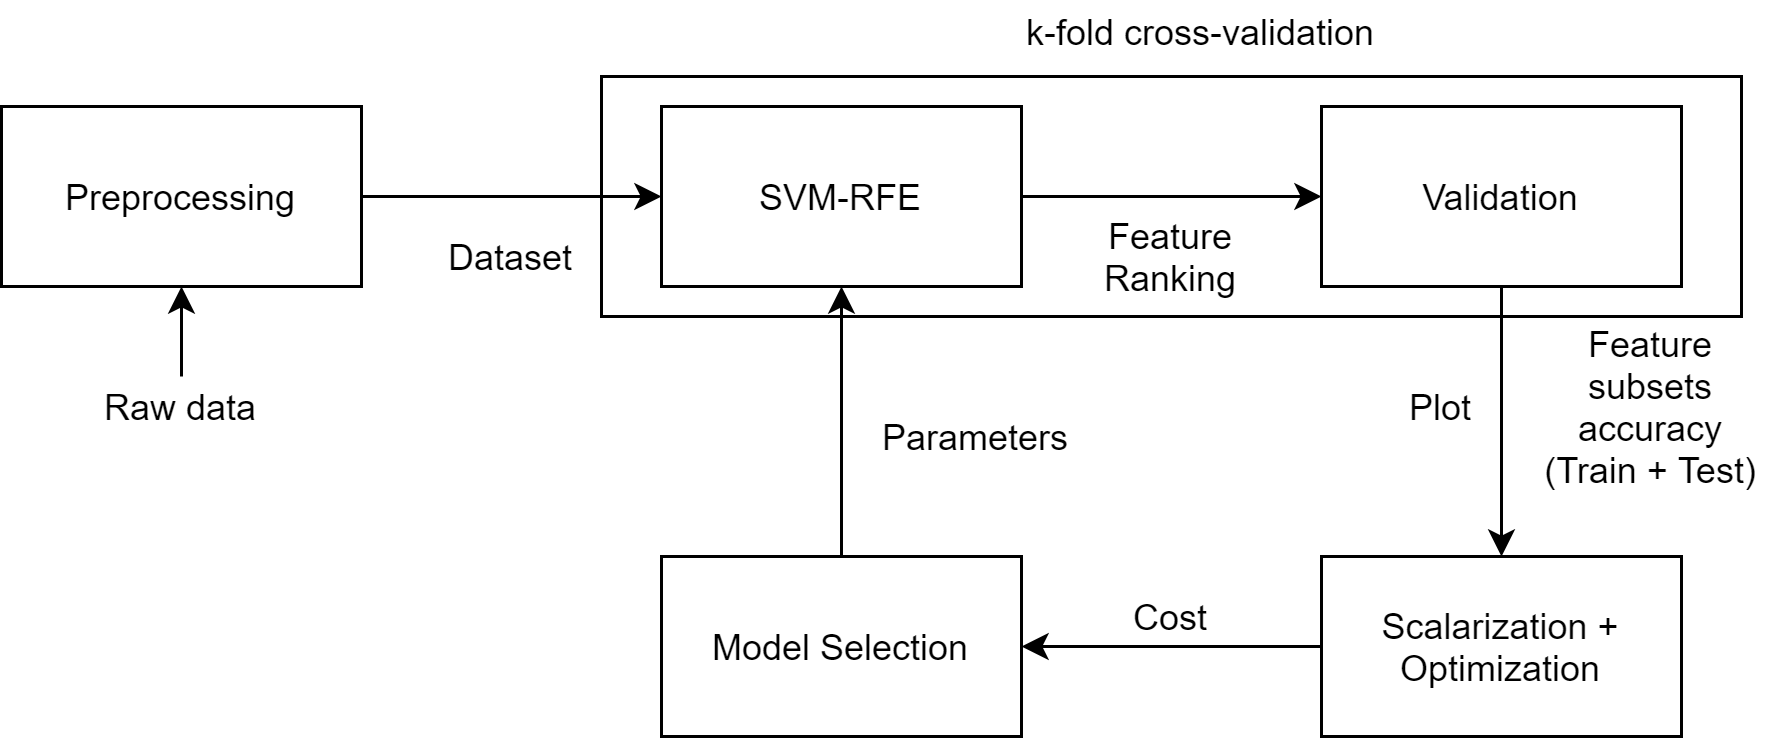
\includegraphics[width=0.8\linewidth]{img/ch5/diag.png}
    \caption{Experimental testing process, divided in phases.}
    \label{fig:ch5.diag}
\end{figure}

\texttt{Sklearn}, being a general machine learning library, has its own implementation of the base \texttt{RFE} algorithm. Given that it is open source, we were able to base our own implementation on it. After pruning the code to its bare minimum (no dep\-en\-den\-cies), we began to add our own extensions. We organized each extension in its own folder, isolated from the rest, and copied the base implementation there.

For the actual experiments we've used \texttt{Jupyter Notebooks} (integrated in \texttt{Visual Studio Code}). Each experiment may use different notebooks depending on what is being tested exactly. Some code that is common to all notebooks, such a code for plotting, has been placed at the beginning (for convenience). The implementation of SVM-RFE and associated usability methods has been moved to separate \texttt{Python} files. This is both a convenient software pattern and a requirement of the parallelization library of our operating system.

We use \emph{k-fold cross-validation} to perform the experiments multiple times with different folds, as explained in section \ref{sec:ch4.performance}. For the same experiment, the same amount of folds is used, but different amounts may be used in different experiments. We've parallelized this procedure with the standard \texttt{multiprocessing.pool} library. Given that our CPU has 8 cores, for the most computationally expensive experiments we're using 6 or 7-fold cross-validation in order to be able to finish the experiment in a single round (with one or two spare cores to be able to keep working in the machine). The execution time is always calculated as the mean of the elapsed times of every SVM-RFE execution (single core).

For plotting we've used the \texttt{Mathplotlib} library. We have made a custom plot function that includes all relevant information for SVM-RFE. Having a standard plot design allows for easy comparison as shown in Figure \ref{fig:ch4.tradeoff}. This plot displays the accuracy (vertical axis) of each feature subset (by size, horizontal axis) based on some feature ranking. We display both the train accuracy and the test accuracy calculated in the validation phase. We also show where the optimal is based on the linear scalarization method. Furthermore, we also show what the minimum accuracy is, based on the amount of classes, with a doted red horizontal line. And finally, we show with an overlay scatter plot of small vertical blue lines, what the actual feature subsets sizes are and what accuracy they had during the execution of SVM-RFE (training accuracy). We can also deduce the step used and the amount of iterations from this information. It is important not to confuse this plot with plots describing an iterative optimization process or model selection.

\subsection{The data}

\subsubsection*{Sklearn Generator}

The general machine learning library \texttt{Sklearn} provides tools to generate artificial datasets for various prob\-lems. We're using the \texttt{make\_classification} gen\-er\-a\-tor, which creates normally-distributed clus\-ters of points placed at the vertices of an hypercube. Multiple clusters can corresponding to a single class. This specific gen\-er\-a\-tor also introduces in\-ter\-de\-pen\-dence between features and var\-i\-ous types of noise.

We've selected this generator because it allows to specify the amount of in\-for\-ma\-tive (i.e. non-redundant, useful) features the dataset should have, it can generate multi-class datasets, and by changing the amount of clusters per class it can control the separability of the data.

We don't use a single dataset of this kind in our experiments. Instead, we use datasets generated with the parameters that we think can better help evaluate the expected properties and correctness of the extensions.

\subsubsection*{MADELON}
\label{sec:ch5.data.madelon}

This is one of the five datasets proposed for the NIPS (Neural Information Processing Systems) 2003 challenge in feature selection. The dataset remains publicly available in the UCI (University of California, Irvine) machine learning repository. The results of this challenge can be found at the workshop web page (\cite{guyon_result_2004}).

The winner of the challenge got an accuracy of 92.89\% with 8 selected features. However, this is using test data that is not publicly available. Using only the avail\-able data we've found articles describing the use of this dataset where the maximum accuracy reached is 88\%. 

This dataset is constructed similarly to the \texttt{sklearn} \texttt{make\_classification} gen\-er\-a\-tor. It uses clusters of points placed at the vertices of some hypercube, however, instead of a single hypercube it uses five of them. Also, this method labels each in hypercube in one of two classes randomly. Five features correspond to the which hypercube a point is in, with an extra 15 being redundant features extracted from linear combinations of the first 5. The total amount of features per data point is 500, 480 of them being noise (also called probes).

Of this dataset, 2000 observations are publicly available and where used in this project, 600 are part of a separate validation set not used in this project, and 1800 are part of a test set not used in this project and also not publicly available. All sets have the same amount of positive and negative samples.

\subsubsection*{Digits}

For the multi-class classification extension we've used the digits dataset (Optical Recognition of Handwritten Digits Data Set). This is also a dataset available in the UCI machine learning repository and is also provided ready to use in \texttt{Sklearn}. This dataset contains 5620 instances of 64 features corresponding to 10 possible handwritten digits. Each feature has been extracted from a 32×32 bitmap by count\-ing the pixels of 4×4 non-overlapping blocks. There are 64 informative features.

For this dataset common accuracy results are around 98\%, but we've found some cases where it can reach 100\%.

\begin{table}
    \centering
    \begin{tabular}{l c c c c}
    \toprule
    \tabhead{Name}      & \tabhead{Observations} & \tabhead{Features} & \tabhead{Informative}& \tabhead{Classes} \\
    \midrule
    \texttt{make\_classification}   & - & - & - & - \\
    MADELON                         & 2000 & 500 & 5 & 2 \\
    Digits                          & 1797 & 64 & ?? & 10 \\
    \bottomrule\\
    \end{tabular}
    \caption{Summary of dataset properties.}
    \label{tab:ch5.datasetdesc}
\end{table}

% -----------------------------------------------------------------------------------------

\section{Dynamic Step}

This extension is based on the constant step variant of SVM-RFE (Algorithm \ref{alg:rfe1}), however, instead of using some constant number $t$ as the step in each iteration, we calculate that number dynamically. The most straightforward way to do this is by using a percentage.

\subsection{Description and reasoning}
\label{sec:dynamicStep.desc}

The percentage is a hyper-parameter. It is used within every iteration to eliminate a number of the least ranked features. A constant step has already been used in pract\-ice, but it is expected that this method will be significantly faster without effecting the accuracy performance, or even improving it.

Other similar modifications are also found in the literature, including using the square root of the remaining features \texttt{SQRT-RFE}, an entropy based function \texttt{E-RFE}, or \texttt{RFE-Annealing} which sets the step at $|\vt{s}| \frac{1}{i+1}$, thus, changing the percentage each iteration (\cite{ding_improving_2006}).

%\iffalse
That is, the amount of features eliminated "$r$" at $j$-th iteration is the summation of the amount of features eliminated each iteration, i.e. $np^i$:

\begin{equation}\label{eq:dynamicStep1}
    r = \sum_{i = 1}^{j}{(np^i)} 
\end{equation}

It may be more interesting to see complexity as in the amount of iterations re\-quired to eliminate $r$ features. Assuming $r$ and $p$ to be constants, it can be derived from equation \ref{eq:dynamicStep1} as follows:

\begin{align*}
    r &= n \sum_{i = 1}^{j}{p^i} = n \sum_{i = 0}^{j-1}{(p^i)} - n + np^j \\
    \frac{r}{n} &= \frac{1-p^j}{1-p} - 1 + p^j \\
    \frac{r}{n} &= \frac{(1-p^j) - (1-p) + (1-p)p^j}{1-p}\\
    \frac{(1-p)r}{n} &= (1-p^j) - (1-p) + (p^j-p^{j+1})\\
    \frac{(1-p)r}{n} &= 1 -p^j -1 + p + p^j - p^{j+1}\\
    \frac{(1-p)r}{n} &= p - p^{j+1}\\
    - \frac{(1-p)r}{n} + p &= p^{j+1}\\
    \log_{p} \left( - \frac{(1-p)r - np}{n} \right) &= \log_{p} (p^{j+1})\\
    \log_{p} \left( - \frac{(1-p)r - np}{n} \right) &= j + 1\\
    \log_{1/p} \left( - \frac{n}{(1-p)r} + 1/p \right) &= j + 1 \implies O(\log_{1/p} n)
\end{align*}\\
%\fi

We assume that, the bigger the step each iteration, the worse the performance of the ranking. This is consistent with what we've seen in figure \ref{fig:ch4.dynamicStep.vanilla.comp}. However, since we're eliminating the worst variables first, eliminating more of them at once shouldn't affect performance because it is likely they would've been eliminated in the next iterations anyway. The fewer the iterations remaining, the riskier it becomes to eliminate multiple variables at once, and thus a smaller step is beneficial.

\subsubsection*{Our expectations for this extension are:}

\begin{itemize}
    \item \textbf{Improvement in time complexity:} Given that SVM complexity $O(mn^2)$ is lin\-ear\-ly dependent on the amount of dimensions $d$, we know that each iteration is faster than the one before it. By increasing the step in the first iterations we should drastically reduce the time it takes to complete, even if then we decide to reduce the step in later, less time-consuming, iterations.
    \item \textbf{Improvement in accuracy performance:} Using dynamic step, compared to a constant step $t > 1$, can also improve the accuracy. This is because the last iterations may be performed with a step $t \ge i \ge 1$.
\end{itemize}

Note that by adjusting the percentage you can decide for which of these two objectives you want to optimize, it may also be possible to find a middle case in which both the accuracy and the time are improved.

\subsection{Pseudocode formalization}

\begin{algorithm}[h]
    \DontPrintSemicolon
      \KwInput{$p$ \tcp*{p = percentage, $0 \le p \le 1$}}
      \KwOutput{$\vt{r}$}
      \KwData{$X_0,\vt{y}$}
      $\vt{s} = [1,2, \dotsc, m]$ \tcp*{subset of surviving features}
      $\vt{r} = []$ \tcp*{feature ranking list} 
      \While{$|\vt{s}| > 0$}
        {
            \tcc*[h]{Restrict training examples to good feature indices}\\
            $X=X_0(:,\vt{s})$\VS

            \tcc*[h]{Train the classifier}\\
            $\vt{\alpha} = \texttt{SVM-train(} X, y \texttt{)}$\VS

            \tcc*[h]{Compute the weight vector of dimension length $|\vt{s}|$}\\
            $\vt{w} = \sum_k{\vt{\alpha_k} \vt{y_k} \vt{x_k}}$\VS

            \tcc*[h]{Compute the ranking criteria}\\
            $\vt{c} = [(w_i)^2 \text{ for all $i$}]$\VS

            \tcc*[h]{Compute $t$ based on the percentage}\\
            $t = p|\vt{s}|$\VS

            \tcc*[h]{Find the $t$ features with the smallest ranking criterion}\\
            $\vt{f} = \texttt{argsort}(\vt{c})(\ :t)$\VS

            \tcc*[h]{Iterate over the feature subset}\\
            \For{$f_i \in \vt{f}$}{
                \tcc*[h]{Update the feature ranking list}\\
                $\vt{r} = [\vt{s}(f_i), ...\vt{r}]$\VS
    
                \tcc*[h]{Eliminate the feature selected}\\
                $\vt{s} = [...\vt{s}(1:f_i - 1), ...\vt{s}(f_i + 1:|\vt{s}|)]$
            }
        }
    \caption{SVM-RFE with DynamicStep}
\end{algorithm}
\VS
Note that since we do a non-lineal skip focused on the iterations that take more time we can achieve a reduced complexity of $O(\log(d)dn^2)$. This can be illustrated in Figure \ref{fig:ch5.dstep.comparetime}, where we show the relationship between the amount of remaining features and iterations for the different step methods. 

\begin{figure}[h]
    \centering
    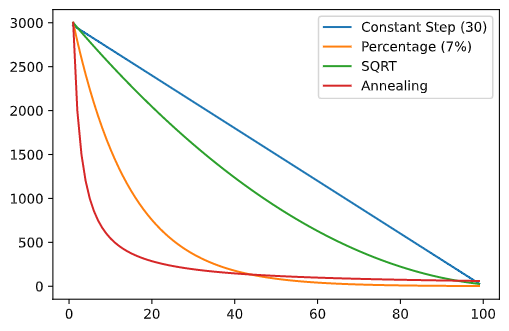
\includegraphics[width=0.4\linewidth]{img/ch5/comparetimes.png}
    \caption{Amount of features remaining (vertical axis) at each iteration (horizontal axis).}
    \label{fig:ch5.dstep.comparetime}
\end{figure}

The relative time cost of each method can be estimated as the area under the curve. Note that in this plot the amount of iterations is fixed, however in practice it may make more sense that dynamic step methods perform much more late iterations than constant step.

\subsection{Results}

\subsubsection*{Analysis with artificially generated data}
\label{sec:ch5.dstep.gen}

We generate a 2 class dataset with the following code. The scalarization trade-off used is of 80\% accuracy, 20\% feature subset size. All results are mean values extracted from a 7-fold cross-validation procedure.

\begin{verbatim}
    X, y = make_classification(
        n_samples = 1000, n_clusters_per_class=3, n_features = 300,
        n_informative = 100, n_redundant=100, n_repeated=20,
        flip_y=0.05, random_state=2, class_sep=2
    )
\end{verbatim}

We start by comparing how the dataset performs under a random feature se\-lec\-tion or a simple filter method. For the validation phase a linear SVM has been used, with the regularization parameter found by grid search and being $C = 0.00001$.

\begin{figure}[H]
    \centering
    \begin{subfigure}[b]{0.4\linewidth}
        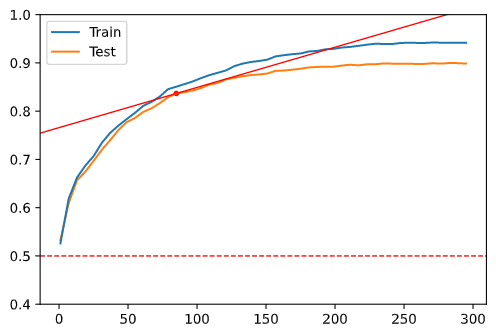
\includegraphics[width=\linewidth]{img/ch5/dstep/random.png}
        \subcaption*{Random AT (85, 0.83, 0.187)}
    \end{subfigure}
    \begin{subfigure}[b]{0.4\linewidth}
        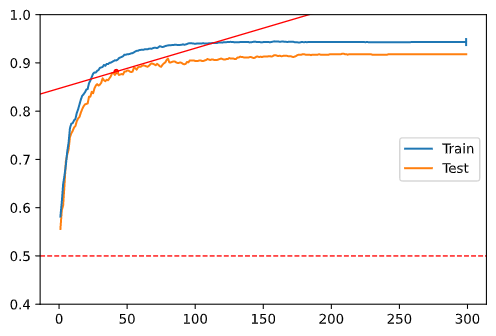
\includegraphics[width=\linewidth]{img/ch5/dstep/filter.png}
        \subcaption*{Filter AT (42, 0.88, 0.122)}
    \end{subfigure}
    \caption{Accuracy of feature rankings produced either by a random method or an SVM-based filter method. AT (\emph{feat.}, \emph{acc.}, \emph{cost})}
    \label{fig:ch5.dstep.init}
\end{figure}

Based on these results we expect that SVM-RFE must perform better than the filter method. Or objective now is to find if using a dynamic step can perform similarly or better than SVM-RFE in less amount of time. From a grid search model selection procedure we'be selected the best feature rankings, shown in Figure \ref{fig:ch5.dstep.vanillabest}.

\begin{figure}[H]
    \centering
    \begin{subfigure}[b]{0.4\linewidth}
        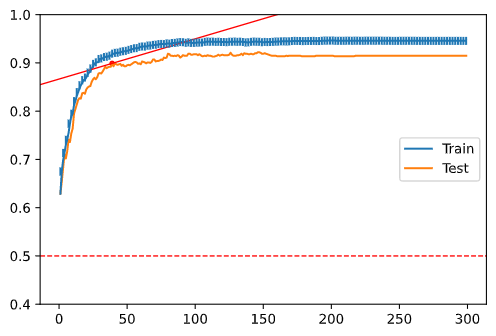
\includegraphics[width=\linewidth]{img/ch5/dstep/vanilla1.png}
        \subcaption*{Const Step $t=2, C=0.00001$}
    \end{subfigure}
    \begin{subfigure}[b]{0.4\linewidth}
        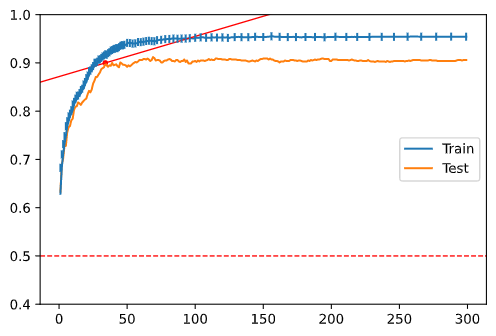
\includegraphics[width=\linewidth]{img/ch5/dstep/vanilla2.png}
        \subcaption*{Dynamic Step $p=0.05, C=0.0001$}
    \end{subfigure}
    \caption{Accuracy of the best feature rankings produced by SVM-RFE with constant or dynamic step.}
    \label{fig:ch5.dstep.vanillabest}
\end{figure}

In the following tables we detail the results of the model selection. The cell corresponding to the best model of each algorithm (by cost) and associated time have been highlighted. 
\begin{table}[H]
    \centering
    \begin{tabular}{l | c c c|c c c|c c c}
        \toprule
        \multicolumn{1}{c}{Step} & \multicolumn{3}{c}{\textbf{2}} & \multicolumn{3}{c}{\textbf{10}} & \multicolumn{3}{c}{\textbf{50}}\\
        %\cline{2-4}\cline{5-7}\cline{8-10}
        \midrule
        \textbf{$C$}&Feat.&Acc.&Cost&Feat.&Acc.&Cost&Feat.&Acc.&Cost \\
        \midrule
        \textbf{0.000001} &    39 & 88.40\% & 0.119 &    41 & 89.40\% & 0.112 &    38 & 88.70\% & 0.116\\
        \textbf{0.000010} &    \mrk{39} & \mrk{89.90\%} & \mrk{0.107} &    57 & 90.70\% & 0.112 &    54 & 89.80\% & 0.118\\
        \textbf{0.000100} &    55 & 91.00\% & 0.109 &    61 & 91.30\% & 0.110 &    59 & 90.10\% & 0.118\\
        \textbf{0.001000} &    81 & 89.40\% & 0.139 &    77 & 87.90\% & 0.148 &    81 & 87.10\% & 0.157\\
        \textbf{0.010000} &   104 & 88.70\% & 0.160 &   103 & 89.10\% & 0.156 &   116 & 87.90\% & 0.174\\
        \bottomrule
        \end{tabular}
    \caption{Grid search of SVM-RFE with constant step.}
\end{table}

\begin{table}[H]
    \centering
    \begin{tabular}{l | c c c}
        \toprule
        \multicolumn{1}{c}{\textbf{C/Step}} & \textbf{2} & \textbf{10} & \textbf{50} \\
        %\cline{2-4}\cline{5-7}\cline{8-10}
        \midrule
        \textbf{0.000001} & 0:03.691 & 0:00.643 & 0:00.124\\
        \textbf{0.000010} & \mrk{0:05.242} & 0:01.050 & 0:00.190\\
        \textbf{0.000100} & 0:07.001 & 0:01.440 & 0:00.279\\
        \textbf{0.001000} & 0:08.039 & 0:01.522 & 0:00.334\\
        \textbf{0.010000} & 0:11.834 & 0:02.424 & 0:00.577\\
        \bottomrule
        \end{tabular}
    \caption{Execution time (min:sec.msec) of SVM-RFE with constant step.}
\end{table}

\begin{table}[H]
    \centering
    \begin{tabular}{l | c c c|c c c|c c c}
        \toprule
        \multicolumn{1}{c}{Percentage} & \multicolumn{3}{c}{\textbf{0.04}} & \multicolumn{3}{c}{\textbf{0.12}} & \multicolumn{3}{c}{\textbf{0.20}}\\
        %\cline{2-4}\cline{5-7}\cline{8-10}
        \midrule
        \textbf{$C$}&Feat.&Acc.&Cost&Feat.&Acc.&Cost&Feat.&Acc.&Cost \\
        \midrule
        \textbf{0.000001} &    26 & 88.20\% & 0.112 &    22 & 86.60\% & 0.122 &    37 & 88.10\% & 0.120\\
        \textbf{0.000010} &    43 & 89.80\% & 0.110 &    36 & 89.80\% & 0.106 &    60 & 89.30\% & 0.126\\
        \textbf{0.000100} &    \mrk{34} & \mrk{90.00\%} & \mrk{0.103} &    59 & 91.00\% & 0.111 &    42 & 90.40\% & 0.105\\
        \textbf{0.001000} &    56 & 87.30\% & 0.139 &    63 & 87.20\% & 0.144 &    91 & 89.00\% & 0.149\\
        \textbf{0.010000} &    87 & 88.40\% & 0.151 &   104 & 87.40\% & 0.170 &   107 & 87.90\% & 0.168\\
        \bottomrule
        \end{tabular}
    \caption{Grid search of SVM-RFE with dynamic step.}
\end{table}

\begin{table}[H]
    \centering
    \begin{tabular}{l | c c c}
        \toprule
        \multicolumn{1}{c}{\textbf{C/Percentage}} & \textbf{0.04} & \textbf{0.12} & \textbf{0.20} \\
        %\cline{2-4}\cline{5-7}\cline{8-10}
        \midrule
        \textbf{0.000001} & 0:01.048 & 0:00.324 & 0:00.202\\
        \textbf{0.000010} & 0:01.455 & 0:00.443 & 0:00.283\\
        \textbf{0.000100} & \mrk{0:01.947} & 0:00.612 & 0:00.380\\
        \textbf{0.001000} & 0:02.505 & 0:00.709 & 0:00.404\\
        \textbf{0.010000} & 0:03.487 & 0:01.079 & 0:00.639\\
        \bottomrule
        \end{tabular}
    \caption{Execution time (min:sec.msec) of SVM-RFE with dynamic step.}
\end{table}

Note that the three best models for dynamic step are all better than the best model using constant step. This results however have to be taken with a grain of salt, given that variance is present and the difference is only marginal.

A more clear-cut improvement can be seen on the computational cost, which had a speedup of x2.7 even when the model used by dynamic step had a greater value of $C$. (Equation \ref{eq:ch5.dstep.speedup1}).
\label{eq:ch5.dstep.speedup1}
\begin{align}
    \text{Speedup} = \frac{T_{\text{old}}}{T_{\text{new}}} = \frac{5.242}{1.947} = 2.692
\end{align}

\begin{verbatim}
    NOTE: The speedup is better the highier the amount of features.
\end{verbatim}


\subsubsection*{Analysis with Madelon}

Like before, we start comparing how the dataset performs under a random ranking (Figure \ref{fig:ch5.dstep.madelon.rand}).

\begin{figure}[H]
    \centering
    \begin{subfigure}[b]{0.4\linewidth}
        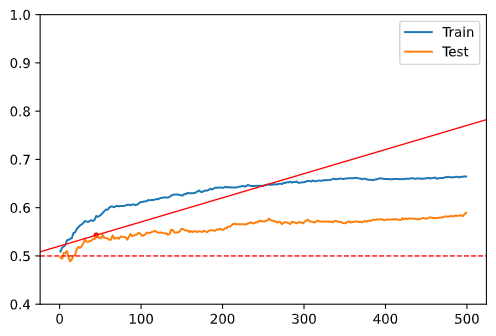
\includegraphics[width=\linewidth]{img/ch5/dstep/madelon-random.png}
        \subcaption*{$C=10^{-5}$}
    \end{subfigure}
    \begin{subfigure}[b]{0.4\linewidth}
        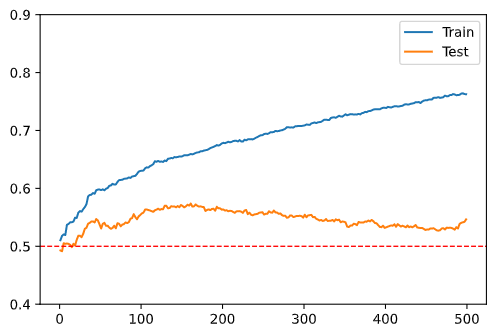
\includegraphics[width=\linewidth]{img/ch5/madelon-random-c_1}
        \subcaption*{$C=10^3$}
    \end{subfigure}
    \caption{Accuracy of an SVM classifier with a random feature selection with the Madelon dataset.}
    \label{fig:ch5.dstep.madelon.rand}
\end{figure}

It seems to perform poorly, even when all features are used. We thought this could be caused by the regularization parameter, so we tried various values of $C$ on a logarithmic scale (Figure \ref{fig:ch5.dstep.madelon.reg}). At first glance, however, it doesn't look like a regularization problem.

\begin{figure}[h]
    \centering
    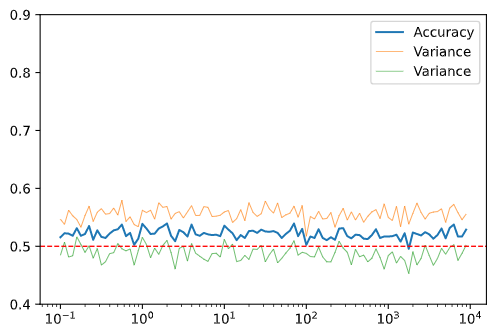
\includegraphics[width=0.4\linewidth]{img/ch5/madelon-cv-c}
    \caption{Hyper-parameter search of $C$. Displaying test accuracy of a linear SVM classifier using all features.}
    \label{fig:ch5.dstep.madelon.reg}
\end{figure}

Next've we've tried to see what happens if we apply normal SVM-RFE directly, with $C=10^{-6}$, see Figure \ref{fig:ch5.dstep.madelon.lin}. Unfortunately, not only is the accuracy much lower than expected (Section \ref{sec:ch5.data.madelon}), but also no improvement can be appreciated when we decrease the step. This indicates that dynamic step will not work, as it relies on this property.

\begin{figure}[h]
    \centering
    \begin{subfigure}[b]{0.4\linewidth}
        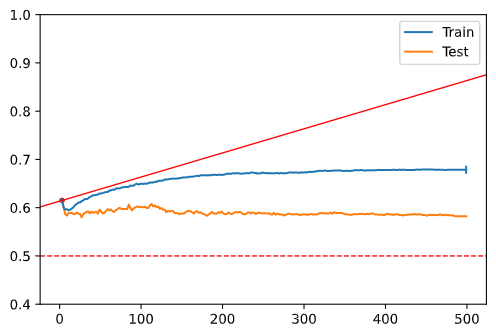
\includegraphics[width=\linewidth]{img/ch5/dstep/madelon-lin1.png}
        \subcaption*{Filter}
    \end{subfigure}
    \begin{subfigure}[b]{0.4\linewidth}
        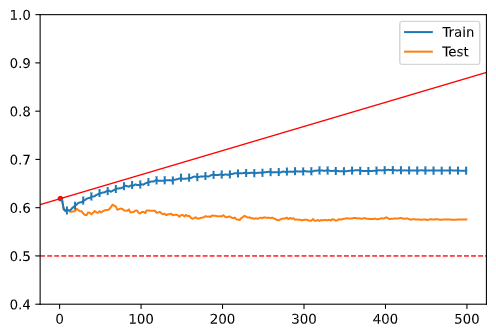
\includegraphics[width=\linewidth]{img/ch5/dstep/madelon-lin2.png}
        \subcaption*{Step = 10}
    \end{subfigure}
    \caption{Accuracy of the ranking produced by SVM-RFE.}
    \label{fig:ch5.dstep.madelon.lin}
\end{figure}

Since the problem is not regularization, then it may be that the data is not linearly separable. Although we can not implement a non-linear kernel for the SVM-RFE procedure yet (it is another extension), we may be able to improve the situation by using a non-lineal kernel on the validation phase (Figure \ref{fig:ch5.dstep.madelon.dyn}).

\begin{figure}[h]
    \centering
    \begin{subfigure}[b]{0.4\linewidth}
        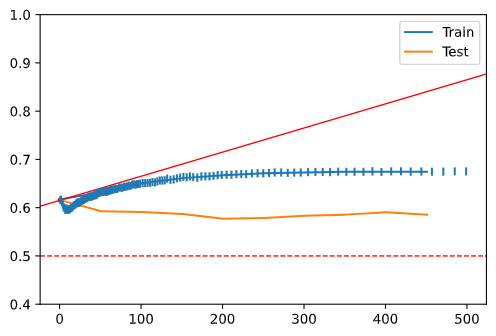
\includegraphics[width=\linewidth]{img/ch5/dstep/madelon-dyn1.png}
        \subcaption*{Lineal, $C = 10^{-6}$}
    \end{subfigure}
    \begin{subfigure}[b]{0.4\linewidth}
        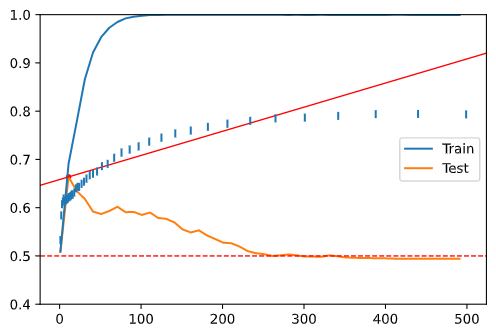
\includegraphics[width=\linewidth]{img/ch5/dstep/madelon-dyn2.png}
        \subcaption*{Polynomial, degree 6, $C = 0.6$}
    \end{subfigure}
    \caption{Accuracy of the ranking produced by a dynamic step SVM-RFE with lineal and polynomial kernels.}
    \label{fig:ch5.dstep.madelon.dyn}
\end{figure}

As expected, dynamic step doesn't improve the accuracy in this scenario. We do see an improvement when using a non-lineal kernel on the validation phase, but again produces the same result as the filter method.

\subsection{Conclusions}

This is a summary of the pros and cons that we've found for this extension:

\begin{itemize}
    \item Using some form of dynamic step may improve the accuracy in certain sce\-nar\-ios, specially in situations where there is a benefit from having a small step.
    \item Using a percentage doesn't introduce a new hyper-parameter since it replaces the existing step constant.
    \item Dynamic step is generally much faster than a constant step for the same levels of accuracy, specially when many features are used and the step is small.
    \item With independence of the accuracy improvement, dynamic step can still be used to speed up considerably the validation phase.
    \item The percentage and final point are better adjusted when the shape of the data is known.
\end{itemize}

In general, we recommend using dynamic step whenever possible, after the initial exploration of the data and if possible after the execution with the associated filter method.

% --------------------------------------------------------------------------------------------------------------------------------------------
% --------------------------------------------------------------------------------------------------------------------------------------------

\section{Sampling}

In this experiment we want to see if using a different subset of observations each iteration can reduce computational cost without negatively affecting performance.

\subsection{Description and reasoning}
\label{sec:ch5.sampling.desc}

Sampling is the process of selecting a representative part of a population. In machine learning sampling is done when creating a dataset, where each observation is a \emph{sample} of some unknown distribution. 

Sampling may also be done, a second time, when preparing the dataset. Clas\-si\-fi\-cation algorithms often require that all classes have a similar number of ob\-ser\-va\-tions, when this condition is not meet it is said that the dataset has \emph{sampling bias}. To avoid sampling bias, the dataset is resampled with another method called \emph{stratified random sampling}. This method consists on making a new dataset with only a subset of the observations, while imposing the restriction that all classes must have the same number of observations.

Because SVM computational cost is directly related to the amount of examples (i.e. samples), using only a subset of observations on each iteration can reduce this cost. In doing that, it is expected that performance will decrease, but we hope that in choosing a different subset each iteration, the performance will increase to levels similar to those we would see while using all data.

The reasoning for this last statement is that, although the algorithm only uses a subset of the data each iteration, by the time the algorithm finishes all data should've been used. Also, it is known that sampling improves generalization, thus we hope that this approx will reduce the gap between test and train error compared to the version with all data.

\subsection{Pseudocode formalization}

\begin{algorithm}[H]
    \DontPrintSemicolon
      \KwInput{$t, k$ \tcp*{$t$ = step, $k$ = number of samples, $0 < k \le |X_0|$}}
      \KwOutput{$\vt{r}$}
      \KwData{$X_0,\vt{y}$}
      $\vt{s} = [1,2, \dotsc, m]$ \tcp*{subset of surviving features}
      $\vt{r} = []$ \tcp*{feature ranked list}
      \While{$|\vt{s}| > 0$}
        {
            \tcc*[h]{Determine subset of examples by random sampling}\\
            $idx = \texttt{random\_sample}(|X_0|, k)$\VS

            \tcc*[h]{Restrict subset of examples to good feature indices}\\
            $X=X_0(idx,\vt{s})$\VS

            \tcc*[h]{Train the classifier}\\
            $\vt{\alpha} = \texttt{SVM-train(} X, y \texttt{)}$\VS

            \tcc*[h]{Compute the weight vector of dimension length $|\vt{s}|$}\\
            $\vt{w} = \sum_k{\vt{\alpha_k} \vt{y_k} \vt{x_k}}$\VS

            \tcc*[h]{Compute the ranking criteria}\\
            $\vt{c} = [(w_i)^2 \text{ for all $i$}]$\VS

            \tcc*[h]{Find the $t$ features with the smallest ranking criterion}\\
            $\vt{f} = \texttt{argsort}(\vt{c})(\ :t)$\VS

            \tcc*[h]{Iterate over the feature subset}\\
            \For{$f_i \in \vt{f}$}{
                \tcc*[h]{Update the feature ranking list}\\
                $\vt{r} = [\vt{s}(f_i), ...\vt{r}]$\VS
    
                \tcc*[h]{Eliminate the feature selected}\\
                $\vt{s} = [...\vt{s}(1:f_i - 1), ...\vt{s}(f_i + 1:|\vt{s}|)]$
            }
        }
    \caption{SVM-RFE with Random Sampling}
\end{algorithm}

\subsection{Results}

\subsubsection*{Analysis with artificially generated data}

We generate a 2 class dataset with the following code. The scalarization trade-off used is 80\% accuracy, 20\% feature subset size. Are results are mean values extracted form a 20-fold cross-validation procedure. For this dataset we've used $C = 10$ across all experiments.

\begin{verbatim}
    X, y = make_classification(
        n_samples = 8000, n_clusters_per_class = 2, n_features = 300, 
        n_informative = 100, n_redundant=2, n_repeated=0,
        flip_y= 0.01, random_state=8, class_sep = 1.0
    )
\end{verbatim}\VS

To test this extension we've created 3 algorithms:

\begin{itemize}
    \item \textbf{A:} No sampling is done, all examples are used as usual.
    \item \textbf{B:} Sampling is done once, as a preprocessing step, not within SVM-RFE.
    \item \textbf{C:} Sampling is done within SVM-RFE, as explained in Section \ref{sec:ch5.sampling.desc}. 
\end{itemize}

Figure \ref{fig:ch5.sampling.vanilla.comp} illustrates the results for 3 different parameter sets (3×3 grid).

\begin{figure}[H]
    \centering
    \begin{subfigure}[b]{0.32\linewidth}
        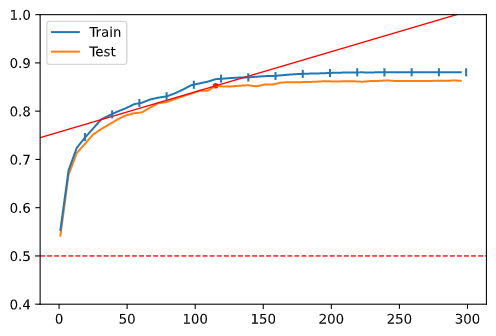
\includegraphics[width=\linewidth]{img/ch5/sampling/300-s20.png}
        \subcaption*{\textbf{A1.} $t = 20$}
    \end{subfigure}
    \begin{subfigure}[b]{0.32\linewidth}
        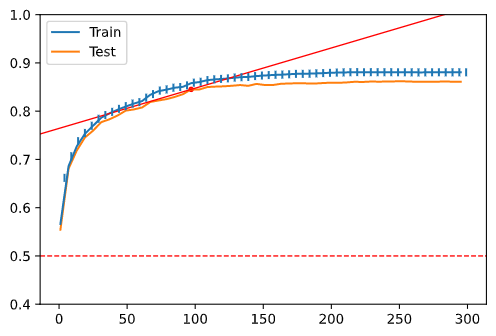
\includegraphics[width=\linewidth]{img/ch5/sampling/300-s5.png}
        \subcaption*{\textbf{A2.} $t = 5$}
    \end{subfigure}
    \begin{subfigure}[b]{0.32\linewidth}
        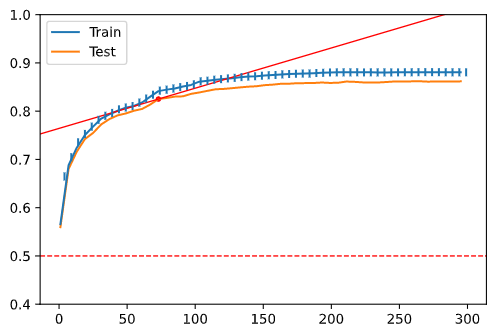
\includegraphics[width=\linewidth]{img/ch5/sampling/300-s5-05v.png}
        \subcaption*{\textbf{A3.} $t = 5$}
    \end{subfigure}
    \begin{subfigure}[b]{0.32\linewidth}
        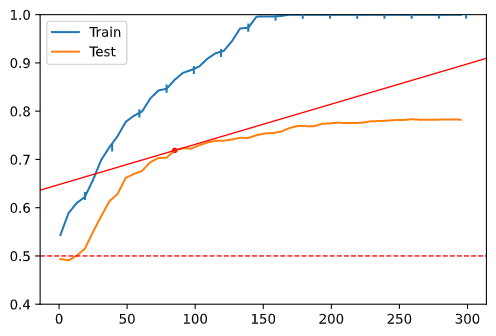
\includegraphics[width=\linewidth]{img/ch5/sampling/300-s20-p01-pre.png}
        \subcaption*{\textbf{B1.} $t = 20, k = 10\%$ PRE}
    \end{subfigure}
    \begin{subfigure}[b]{0.32\linewidth}
        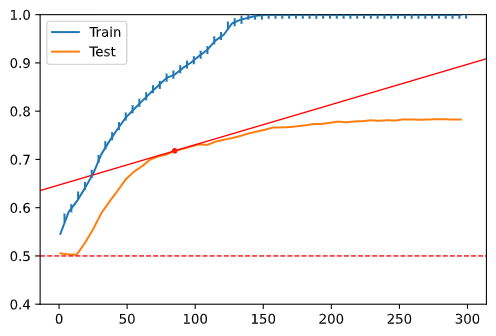
\includegraphics[width=\linewidth]{img/ch5/sampling/300-s5-p01-pre.png}
        \subcaption*{\textbf{B2.} $t = 5, k = 10\%$ PRE}
    \end{subfigure}
    \begin{subfigure}[b]{0.32\linewidth}
        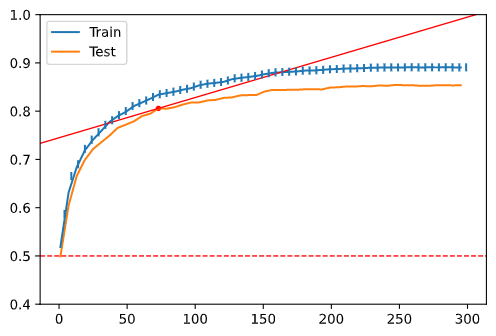
\includegraphics[width=\linewidth]{img/ch5/sampling/300-s5-p05-pre.png}
        \subcaption*{\textbf{B3.} $t = 5, k = 50\%$ PRE}
    \end{subfigure}
    \begin{subfigure}[b]{0.32\linewidth}
        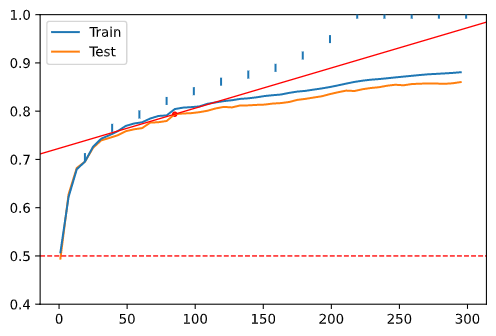
\includegraphics[width=\linewidth]{img/ch5/sampling/300-s20-p01.png}
        \subcaption*{\textbf{C1.} $t = 20, k = 10\%$}
    \end{subfigure}
    \begin{subfigure}[b]{0.32\linewidth}
        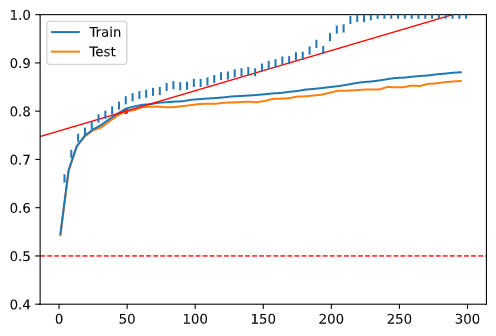
\includegraphics[width=\linewidth]{img/ch5/sampling/300-s5-p01.png}
        \subcaption*{\textbf{C2.} $t = 5, k = 10\%$}
    \end{subfigure}
    \begin{subfigure}[b]{0.32\linewidth}
        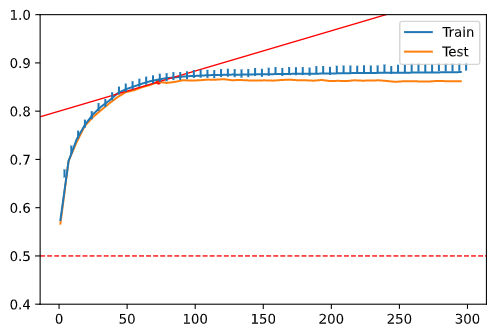
\includegraphics[width=\linewidth]{img/ch5/sampling/300-s5-p05.png}
        \subcaption*{\textbf{C3.} $t = 5, k = 50\%$}
    \end{subfigure}
    \caption{Grid comparing algorithms on each row \textbf{A-B-C} and the hyper-parameter configuration for each \textbf{1} (step = 20), \textbf{2} (step = 5, sample = 10\%) and \textbf{3} (step = 5, sample = 50\%).}
    \label{fig:ch5.sampling.vanilla.comp}
\end{figure}

\begin{table}[h]
    \centering
    \begin{tabular}{l | c c c|c c c|c c c}
        \toprule
        \multicolumn{1}{c}{} & \multicolumn{3}{c}{\textbf{1}} & \multicolumn{3}{c}{\textbf{2}} & \multicolumn{3}{c}{\textbf{3}}\\
        %\cline{2-4}\cline{5-7}\cline{8-10}
        \midrule
        &Feat.&Acc.&Score&Feat.&Acc.&Score&Feat.&Acc.&Score \\
        \midrule
        \textbf{A}&      115 & 85.25\% & 0.194 &      97 & 84.51\% & 0.189 &     73 & 82.51\% & 0.189\\
        \textbf{B}&      85 & 71.88\% & 0.281 &       85 & 71.79\% & 0.282 &     73 & 80.58\% & 0.204\\
        \textbf{C}&      85 & 79.38\% & 0.221 &       49 & 79.99\% & 0.193 &     \mrk{73} & \mrk{86.08\%} & \mrk{0.160}\\
        \bottomrule
        \end{tabular}
    \caption{Perfomrance.}
\end{table}

\begin{table}[h]
    \centering
    \begin{tabular}{l | c c c | c c c | c c c }
        \toprule
        \multicolumn{1}{c}{} &\multicolumn{3}{c}{\textbf{1}} & \multicolumn{3}{c}{\textbf{2}} & \multicolumn{3}{c}{\textbf{3}}\\
        %\cline{2-4}\cline{5-7}\cline{8-10}
        \midrule
        &Iter.&Time ($s$) &Var. ($s^2$)&Iter.&Time ($s$) &Var. ($s^2$)&Iter.&Time ($s$) &Var. ($s^2$) \\
        \midrule
        \textbf{A}&      15 & 07.82 & 0.26 &      60 & 30.35 & 7.68 &     60 & 30.87 & 2.21\\
        \textbf{B}&      15 & 01.46 & 0.16 &      60 & 05.29 & 1.86 &     60 & 16.26 & 4.70\\
        \textbf{C}&      15 & 03.18 & 2.14 &      60 & 13.43 & 5.51 &     \mrk{60} & \mrk{19.64} & \mrk{1.75}\\
        \bottomrule
        \end{tabular}
    \caption{Times.}
\end{table}

Note how algorithm \textbf{C} performs significatively better than \textbf{B} for all parameter sets, although it takes a bit more time. This extra time consumption can be attributed to the resampling procedure being performed each iteration of SVM-RFE versus only once. This will only be noticeable when the amount of samples is big. However, algorithm \textbf{C} is always faster than algorithm \textbf{A} and even performs better in one parameter set.

\subsubsection*{Analysis with artificially generated data 2}

We've recycled the dataset generated for the dynamic step extension (Section \ref{sec:ch5.dstep.gen}) and repeated the experiment using the same parameters, including the 7-fold cross-validation and fixing a constant step of 10. The fol\-low\-ing tables summarize the result.

\begin{table}[H]
    \centering
    \begin{tabular}{l | c c c|c c c|c c c}
        \toprule
        \multicolumn{1}{c}{Percentage} & \multicolumn{3}{c}{\textbf{1.0}} & \multicolumn{3}{c}{\textbf{0.5}} & \multicolumn{3}{c}{\textbf{0.2}}\\
        %\cline{2-4}\cline{5-7}\cline{8-10}
        \midrule
        \textbf{$C$}&Feat.&Acc.&Cost&Feat.&Acc.&Cost&Feat.&Acc.&Cost \\
        \midrule
        \textbf{0.000010} &    \mrk{37} & \mrk{89.50\%} & \mrk{0.109} &    55 & 88.70\% & 0.127 &    43 & 84.10\% & 0.156\\
        \textbf{0.000100} &    37 & 89.50\% & 0.109 &    37 & 87.50\% & 0.125 &    43 & 82.20\% & 0.171\\
        \textbf{0.001000} &    85 & 88.10\% & 0.152 &    37 & 85.20\% & 0.143 &    37 & 79.11\% & 0.192\\
        \textbf{0.010000} &   103 & 85.30\% & 0.186 &    67 & 85.10\% & 0.164 &    13 & 75.99\% & 0.201\\
        \textbf{0.100000} &    85 & 84.00\% & 0.185 &    67 & 84.90\% & 0.165 &    19 & 78.00\% & 0.189\\
        \bottomrule
        \end{tabular}
    \caption{Grid search of SVM-RFE with preprocessed sampling.}
\end{table}

\begin{table}[H]
    \centering
    \begin{tabular}{l | c c c}
        \toprule
        \multicolumn{1}{c}{\textbf{C/Percentage}} & \textbf{1.0} & \textbf{0.5} & \textbf{0.2} \\
        %\cline{2-4}\cline{5-7}\cline{8-10}
        \midrule
        \textbf{0.000010} & \mrk{0:00.972} & 0:00.308 & 0:00.119\\
        \textbf{0.000100} & 0:01.249 & 0:00.422 & 0:00.166\\
        \textbf{0.001000} & 0:01.799 & 0:00.497 & 0:00.481\\
        \textbf{0.010000} & 0:02.604 & 0:02.106 & 0:02.492\\
        \textbf{0.100000} & 0:09.914 & 0:02.279 & 0:00.207\\
        \bottomrule
        \end{tabular}
    \caption{Execution time (min:sec.msec) of SVM-RFE with pre\-processed sampling.}
\end{table}

\begin{table}[H]
    \centering
    \begin{tabular}{l | c c c|c c c|c c c}
        \toprule
        \multicolumn{1}{c}{Percentage} & \multicolumn{3}{c}{\textbf{0.5}} & \multicolumn{3}{c}{\textbf{0.2}} & \multicolumn{3}{c}{\textbf{0.1}}\\
        %\cline{2-4}\cline{5-7}\cline{8-10}
        \midrule
        \textbf{$C$}&Feat.&Acc.&Cost&Feat.&Acc.&Cost&Feat.&Acc.&Cost \\
        \midrule
        \textbf{0.000010} &    31 & 85.20\% & 0.139 &    37 & 86.20\% & 0.135 &    67 & 88.01\% & 0.141\\
        \textbf{0.000100} &    55 & 90.10\% & 0.116 &    43 & 89.70\% & 0.111 &    73 & 90.00\% & 0.129\\
        \textbf{0.001000} &    \mrk{37} & \mrk{90.30\%} & \mrk{0.102} &    49 & 89.90\% & 0.113 &    49 & 88.60\% & 0.124\\
        \textbf{0.010000} &    49 & 90.20\% & 0.111 &    49 & 89.00\% & 0.121 &    49 & 87.20\% & 0.135\\
        \textbf{0.100000} &    37 & 88.30\% & 0.118 &    55 & 86.70\% & 0.143 &    43 & 85.90\% & 0.141\\
        \bottomrule
        \end{tabular}
    \caption{Grid search of SVM-RFE with sampling.}
\end{table}

\begin{table}[H]
    \centering
    \begin{tabular}{l | c c c}
        \toprule
        \multicolumn{1}{c}{\textbf{C/Percentage}} & \textbf{0.5} & \textbf{0.2} & \textbf{0.1} \\
        %\cline{2-4}\cline{5-7}\cline{8-10}
        \midrule

        \textbf{0.000010} & 0:00.303 & 0:00.130 & 0:00.101\\
        \textbf{0.000100} & 0:00.315 & 0:00.129 & 0:00.097\\
        \textbf{0.001000} & \mrk{0:00.331} & 0:00.145 & 0:00.098\\
        \textbf{0.010000} & 0:00.376 & 0:00.166 & 0:00.114\\
        \textbf{0.100000} & 0:00.499 & 0:00.262 & 0:00.170\\
        \bottomrule
        \end{tabular}
    \caption{Execution time of SVM-RFE with sampling.}
\end{table}

We see similar results in this experiment, reaching both better performance and time even compared to the version without sampling (percentage of 100\%). We note that the best regularization parameter $C$ is kept the same when using preprocessed sampling, yet it is shifted when using sampling within RFE.

\subsubsection*{Analysis with Madelon}

We've tested this extension with the Madelon dataset, but we've obtained similar results as in the previous extension. That is, there is no improvement in accuracy compared to the filter version. This makes using any kind of sampling non-practical given that if only one iteration is done then sampling outside or inside SVM-RFE are equivalent. Furthermore, outside sampling produces worse results.

\subsection{Conclusions}

This is a summary of the pros and cons we've found for this extension:

\begin{itemize}
    \item It is always faster than using no sampling, but slower than using sampling as a preprocessing step.
    \item It generally performs much better than using a preprocessed sampling, and may even improve on the performance of the version with no sampling.
    \item Its performance depends on the amount of iterations, improving the more there are and being equivalent to preprocessed sampling for the filter case.
\end{itemize}

In general, we recommend using SVM-RFE with sampling whenever possible, specially to improve the speed of the algorithm.

% --------------------------------------------------------------------------------------------------------------------------------------------
% --------------------------------------------------------------------------------------------------------------------------------------------

\section{Stop Condition}

This modification intends to find an approximation to the optimal feature subset size within the SVM-RFE phase. This information allows using dynamic step more effectively. Using this extension we don't require a validation phase, which makes it very computationally efficient.

\subsection{Description and reasoning}
\label{sec:ch5.stopcond.desc}

\subsubsection*{Relationship with \emph{Dynamic Step}}

We had some previous success with the \emph{dynamic step} extension. One problem with that extension, however, is that it functions better when the number of informative features is known. By default, \emph{dynamic step} reduces the step size the fewer features are left remaining. This generally improves performance since bigger steps (i.e. fewer iterations) are used in the more computationally expensive parts of the al\-go\-rithm and smaller steps are used on a less expensive region. 

Because smaller steps also imply an improvement in accuracy, we would want to concentrate them on the most critical region of our feature subset space, that is, around the optimal feature subset size. We can easily modify our implementation of \emph{Dynamic Step} so that it is centered at this point by applying our percentage on the distance to that point instead of the amount of remaining features. This time, since this point may be in a region that is more computationally expensive, we may also want to specify a minimum step parameter. Equation \ref{eq:ch5.stopcond.dyns} combines these ideas. Where $p$ is the percentage, $min$ is the minimum step, $c$ is the optimal feature subset size and $i$ is the amount of remaining features.
\begin{align}
    t = \max(p|c-i|, min)
    \label{eq:ch5.stopcond.dyns}
\end{align}

Figure \ref{fig:ch5.stopcond.lines} adds the new method to the dynamic step formulations described in the \emph{Dynamic Step} extension (Figure \ref{fig:ch5.dstep.comparetime}). Note that for the left plot the slope of the curve corresponds with the step used in that iteration. The area under the curve is an approximation of the computational cost. For the left plot, the areas below the constant step line correspond to regions where, due to a smaller step, an increase in accuracy for that feature subset is possible. This, however, will only be useful in practice if that region is within the optimal feature subset size (red doted line).

\begin{figure}[h]
    \centering
    \begin{subfigure}[b]{0.4\linewidth}
        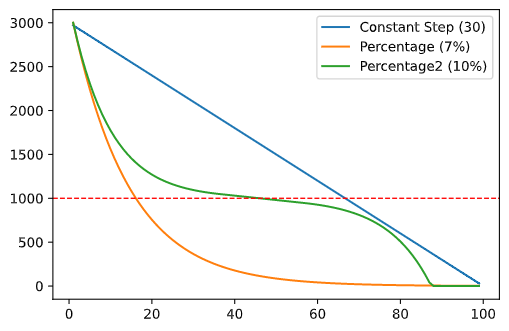
\includegraphics[width=\linewidth]{img/ch5/stopcond/lines.png}
        \subcaption*{Features remaining (vertical axis) at each iteration (horizontal axis).}
    \end{subfigure}
    \hspace{0.05\linewidth}
    \begin{subfigure}[b]{0.4\linewidth}
        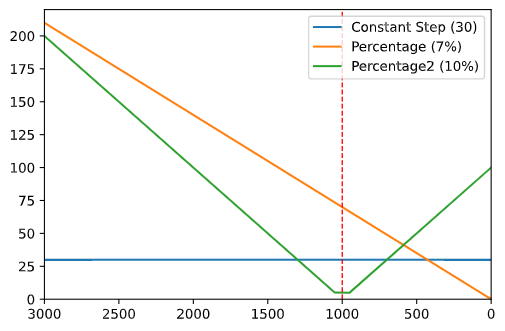
\includegraphics[width=\linewidth]{img/ch5/stopcond/lines2.png}
        \subcaption*{Step (vertical axis) for each feature subset size (horizontal axis).}
    \end{subfigure}
    \caption{ The new method “Percentage2” has a much smaller slope/step at the optimal feature subset size (1000).}
    \label{fig:ch5.stopcond.lines}
\end{figure}

\subsubsection*{Estimating the optimal feature subset size}

There are multiple ways to estimate this point. Of course, running a whole cycle of SVM-RFE and validation (refer to figure \ref{fig:ch5.diag}) and calculating the optimal feature subset size is always an option. However, doing this previously to the SVM-RFE phase for every hyper-parameter set would be very expensive and completely defeat the purpose (since it would be more expensive than using constant step). Another option is to use the amount of informative features as an approximation (this is what we do in the \emph{Combo} experiments), however this information is not always available.

If we're running a model selection process, it may be good enough to simply run a whole cycle once (with constant step), extract the optimal feature subset size for that hyper-parameter configuration and use it as an estimate for the rest. This, however, requires to make an initial run while guessing the hyper-parmaters, and it needs to perform reasonably well. 

We may have better luck by doing an initial grid search under simplified datasets (such as with sampling or a big constant step on SVM-RFE). This, however, may still take a con\-sid\-er\-able amount of time (due to validation requiring a small step) and the results can still not extrapolate well to the full version (since an extreme reduction in sample size may induce shifts on the accuracy distribution of feature subsets).

\subsubsection*{Approximating accuracy by feature importance}

The idea is to approximate the optimal feature subset size based on information we already have within SVM-RFE. Specifically, we want to use the feature importance calculated with the ranking criteria as an estimator of accuracy. This has the ad\-van\-tage that the whole validation phase can be skipped while hopefully still retaining a good approximation. It is also important that the same scalarization trade-off can be used here as well.

We assume that the importance of a feature is directly correlated with the error that is generated when the feature is removed. The total error generated for some feature subset can then be calculated as the commutative sum of the im\-por\-tances for all removed features up to that point. We then scale this result to be between 0.5 and 1.0.

Instead of scaling between two fix values we can get a better approximation by making use of RFE iterations. Each iteration we perform a small testing round (only with training data) to get a true training accuracy. We can then scale our approximation within the bounds of these values. Note that we could also linearly interpolate between this known values and get similar results, without a validation phase. This would however require small values for the step. The beauty of this method is that it still works even when the step used is large (or even equal to the amount of features).

\subsection{Pseudocode formalization}

\begin{algorithm}[H]
    \DontPrintSemicolon
      \KwInput{$t, t_0$ \tcp*{$t$ = step, $t_0$ = threshold, $0 \le t_0$}}
      \KwOutput{$\vt{r}, \vt{q}$}
      \KwData{$X_0,\vt{y}$}
      $\vt{s} = [1,2, \dotsc, m]$ \tcp*{subset of surviving features}
      $\vt{r} = []$ \tcp*{feature ranking list}
      $\vt{q} = []$ \tcp*{accuracy estimators}
      \While{$|\vt{s}| > 0$}
        {
            \tcc*[h]{Restrict training examples to good feature indices}\\
            $X=X_0(:,\vt{s})$\VS

            \tcc*[h]{Train the classifier}\\
            $\vt{\alpha} = \texttt{SVM-train(} X, y \texttt{)}$\VS

            \tcc*[h]{Compute the weight vector of dimension length $|\vt{s}|$}\\
            $\vt{w} = \sum_k{\vt{\alpha_k} \vt{y_k} \vt{x_k}}$\VS

            \tcc*[h]{Compute the ranking criteria}\\
            $\vt{c} = [(w_i)^2 \text{ for all $i$}]$\VS

            \tcc*[h]{Find the $t$ features with the smallest ranking criterion}\\
            $\vt{f} = \texttt{argsort}(\vt{c})(\ :t)$\VS

            \tcc*[h]{Iterate over the feature subset}\\
            \For{$f_i \in \vt{f}$}{
                \tcc*[h]{Append importance of the feature to be eliminated}\\
                $\vt{q} = [\vt{c}(f_i), ...\vt{q}]$\VS
    
                \tcc*[h]{Update the feature ranking list}\\
                $\vt{r} = [\vt{s}(f_i), ...\vt{r}]$\VS
    
                \tcc*[h]{Eliminate the feature selected}\\
                $\vt{s} = [...\vt{s}(1:f_i - 1), ...\vt{s}(f_i + 1:|\vt{s}|)]$
            }
        }
    \caption{SVM-RFE with Stop Condition}
    \label{alg:svmrfe.stopcond}
\end{algorithm}\VS\VS

\begin{algorithm}
    \DontPrintSemicolon
      \KwInput{$\vt{q}, min, max, w_1, w_2$ \tcp*{$\vt{q}$ = importance estimators \\ $w_0, w_1$ = scalarization coef.}}
      \KwOutput{$\text{arg} \min \vt{c}$}
      $\vt{c} = []$ \tcp*{list of cost of every feature subset}
      $\vt{s}$ \quad s.t. \quad $s_i = \sum_{i = 1}^k q_k$\VS
      
      \For{$e_i \in \vt{s}$}
        {
            \tcc*[h]{Estimate the accuracy from the cumulative importance}\\
            $\texttt{Acc} = (1 - e / \max(\vt{s})) / (max - min) + min$\VS

            \tcc*[h]{Scalarization}\\
            $c_i = w_1 (1 - \texttt{Acc}) + w_2 (i / |\vt{s}|)$
        }
    \caption{Stop Point Extraction}
    \label{alg:svmrfe.stopcond.extract}
\end{algorithm}

\subsection{Results}

\subsubsection*{Analysis with artificially generated data}

We reuse the 2 class dataset from the \emph{Dynamic Step} extension. The scalarization trade-off used is 80\% accuracy, 20\% feature subset size. All results are mean values extracted form a 7-fold cross-validation procedure.

\begin{verbatim}
    X, y = make_classification(
        n_samples = 1000, n_clusters_per_class = 3, n_features = 300, 
        n_informative = 100, n_redundant=100, n_repeated=20,
        flip_y= 0.05, random_state=2, class_sep = 2.0
    )
\end{verbatim}\VS

Plot \ref{fig:ch5.stopcond.main} illustrates our algorithm. The green line is our (train) accuracy estimate. We estimate the optimal feature subset size (green dot) and compare it to the true optimal (red dot) found by doing a full SVM-RFE and validation cycle using a much smaller step.

\begin{figure}[h]
    \centering
    \begin{subfigure}[b]{0.4\linewidth}
        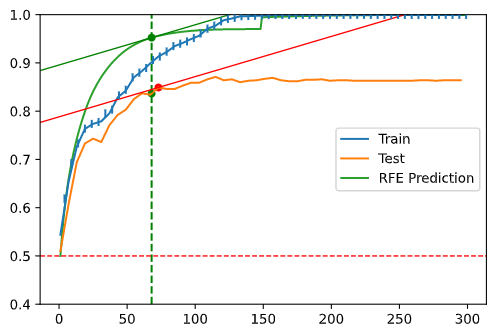
\includegraphics[width=\linewidth]{img/ch5/stopcond/aprox-good.png}
        \subcaption*{Step = 150. Good.}
    \end{subfigure}
    \begin{subfigure}[b]{0.4\linewidth}
        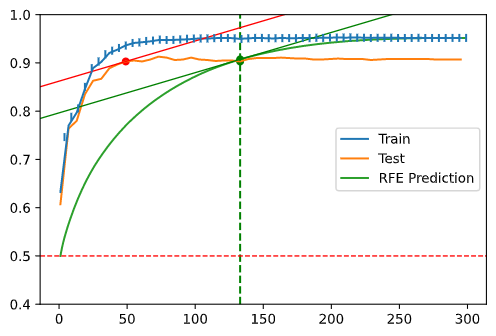
\includegraphics[width=\linewidth]{img/ch5/stopcond/aprox-bad.png}
        \subcaption*{Step = 300. Bad.}
    \end{subfigure}
    \caption{Accuracy estimation (green) for feature ranking generated with SVM-RFE with a step of 10.}
    \label{fig:ch5.stopcond.main}
\end{figure}

\begin{table}[h]
    \centering
    \makebox[0cm]{
    \begin{tabular}{l | c c c|c c c|c c c}
        \toprule
        \multicolumn{1}{c}{Step} & \multicolumn{3}{c}{\textbf{300}} & \multicolumn{3}{c}{\textbf{150}} & \multicolumn{3}{c}{\textbf{60}}\\
        %\cline{2-4}\cline{5-7}\cline{8-10}
        \midrule
        \textbf{$C$}&Opt.&Est.&Diff.&Opt.&Est.&Diff.&Opt.&Est.&Diff. \\
        \midrule
        \textbf{0.00001} &   43 & 104 & 61 &   31 & 105 & 74 &   43 & 58 & 15\\
        \textbf{0.00010} &   49 & 133 & 84 &   37 & 108 & 71 &   55 & 50 & 5\\
        \textbf{0.00100} &   97 & 123 & 26 &   73 & 93 & 20 &   67 & 80 & 13\\
        \textbf{0.01000} &   73 & 66 & 7 &   97 & 80 & 17 &   103 & 119 & 16\\
        \textbf{0.10000} &   73 & 60 & 13 &   79 & 71 & 8 &   73 & 119 & 46\\
        \bottomrule
    \end{tabular}
    }
    \caption{Grid search of SVM-RFE with multi. The cost includes standard error.}
    \label{fig:ch5.stopcond.table}
\end{table}

\begin{table}[h]
    \centering
    \makebox[0cm]{
    \begin{tabular}{l | c c c|c c c|c c c}
        \toprule
        \multicolumn{1}{c}{Step} & \multicolumn{3}{c}{\textbf{300}} & \multicolumn{3}{c}{\textbf{150}} & \multicolumn{3}{c}{\textbf{60}}\\
        %\cline{2-4}\cline{5-7}\cline{8-10}
        \midrule
        \textbf{$C$}&Opt.&Est.&Diff.&Opt.&Est.&Diff.&Opt.&Est.&Diff. \\
        \midrule
        \textbf{0.00001} &   14.3\% & 34.7\% & 20.3\% &   10.3\% & 35.0\% & 24.7\% &   14.3\% & 19.3\% & 5.0\%\\
        \textbf{0.00010} &   16.3\% & 44.3\% & 28.0\% &   12.3\% & 36.0\% & 23.7\% &   18.3\% & 16.7\% & 1.7\%\\
        \textbf{0.00100} &   32.3\% & 41.0\% & 8.7\% &   24.3\% & 31.0\% & 6.7\% &   22.3\% & 26.7\% & 4.3\%\\
        \textbf{0.01000} &   24.3\% & 22.0\% & 2.3\% &   32.3\% & 26.7\% & 5.7\% &   34.3\% & 39.7\% & 5.3\%\\
        \textbf{0.10000} &   24.3\% & 20.0\% & 4.3\% &   26.3\% & 23.7\% & 2.7\% &   24.3\% & 39.7\% & 15.3\%\\
        \bottomrule
    \end{tabular}
    }
    \caption{Grid search of SVM-RFE with multi. The cost includes standard error.}
    \label{fig:ch5.stopcond.table2}
\end{table}

\begin{table}[H]
    \centering
    \begin{tabular}{l | c c c | c c c}
        \toprule
         & \multicolumn{3}{c}{\textbf{Estimate}} & \multicolumn{3}{c}{\textbf{SVM-RFE (Step = 10)}} \\
        %\cline{2-4}\cline{5-7}\cline{8-10}
        \midrule
        \textbf{$C$/Step.}&\textbf{1.0}&\textbf{0.5}&\textbf{0.2}&\textbf{1.0}&\textbf{0.5}&\textbf{0.2} \\
        \midrule
        \textbf{0.00001} & 0:00.095 & 0:00.098 & 0:00.211 &     0:02.276 & 0:02.070 & 0:02.222\\
        \textbf{0.00010} & 0:00.112 & 0:00.143 & 0:00.275 &     0:02.907 & 0:02.897 & 0:02.870\\
        \textbf{0.00100} & 0:00.118 & 0:00.173 & 0:00.350 &     0:03.069 & 0:03.156 & 0:03.329\\
        \textbf{0.01000} & 0:00.213 & 0:00.300 & 0:00.520 &     0:04.428 & 0:05.253 & 0:05.015\\
        \textbf{0.10000} & 0:01.068 & 0:01.173 & 0:02.380 &     0:16.667 & 0:20.553 & 0:21.317\\
        \bottomrule
        \end{tabular}
    \caption{Execution time of SVM-RFE with non-linear kernels.}
    \label{fig:ch5.stopcond.art.tabletime}
\end{table}

\subsection{Conclusions}

This is a summary of the pros and cons we've found for this extension:

\begin{itemize}
    \item It often works. Even when we only do one or two iterations the approximation is often quite close (<10\%) the true optimal feature subset size.
    \item It doesn't always work. Even when we do use five iterations we may still get quite bad (>10\%) approximations for certain parameter configurations.
    \item It's fast. One run takes roughly only 1/20 of the total time a normal SVM-RFE run would take, and completely skips validation.
\end{itemize}

In general, we recommend using it when the amount of informative features is not known. We can integrate it with the model selection to automatically find what the optimal feature subset size is and use the extensions that require such information.

% --------------------------------------------------------------------------------------------------------------------------------------------
% --------------------------------------------------------------------------------------------------------------------------------------------


\section{Multi-Class}

In this section we extend SVM-RFE to the multi-class classification problem.

\subsection{Description and reasoning}
\label{sec:stopCond.desc}

When it comes to extending SVM to handle a multi-class problem two common methods exists, OvR (One-vs-Rest) and OvO (One-vs-One). In both cases the idea is to divide the problem in a set of binary classification problems. Then we use a joint decision function that operates on the results of each pair of problems. Because we're not really making any predictions during the SVM-RFE phase, we can not use this joint decision function. Instead, we must find a way to merge the feature rankings obtained from each problem, i.e. find a joint ranking criteria.

We know that the ranking criteria is an estimator of the importance of some feature for a given binary decision problem. It can be the case that a feature is very useful to distinguish between two classes but useless for the rest. In this case a joint ranking criteria formed by taking the mean, the median or the sum will result in poor selections. A better idea would be to take the maximum. However, it may also be desirable to estimate the joint importance a feature has. For that we may want to consider its individual importance in more than one problem. That is, a feature that is important in more than one pair is more relevant than another that is only important in one such pair, even when the second importance value is greater. A way to perform such ranking would be, for instance, the sum of the squares.

Note that \texttt{sklearn} only supports OvO, and is therefore the option we will use.

\subsection{Pseudocode formalization}

\begin{algorithm}[H]
    \DontPrintSemicolon
      \KwInput{$t, k$ \tcp*{$t$ = step, $k$ = degree}}
      \KwOutput{$\vt{r}$}
      \KwData{$\chi_0,\vt{\psi}$}
      $\vt{s} = [1,2, \dotsc, m]$ \tcp*{subset of surviving features}
      $\vt{r} = []$ \tcp*{feature ranking list}
      \While{$|\vt{s}| > 0$}
        {
            \tcc*[h]{Restrict training examples to good feature indices}\\
            $\chi = \chi_0(:,\vt{s})$\VS

            \tcc*[h]{Compute the joint ranking criteria}\\
            $C = [[], ...]$\\
            \For{$X \subseteq \chi$, $\vt{y} \subseteq \vt{\psi}$ with $X$ and $\vt{y}$ being an instance of OvO}{
                \tcc*[h]{Train the classifier}\\
                $\vt{\alpha} = \texttt{SVM-train(} X, \vt{y} \texttt{)}$\VS

                \tcc*[h]{Compute the weight vector of dimension length $|\vt{s}|$}\\
                $\vt{w} = \sum_k{\vt{\alpha_k} \vt{y_k} X_k}$\VS
    
                \tcc*[h]{Append feature importance list}\\
                $C = [...C, [(w_i)^2 \text{ for all } i ]]$\VS
            }\VS

            \tcc*[h]{Join feature importances}\\
            $\vt{c} = \underset{j}{\sum} C_{i,j}^k \text{ for all } i$\VS

            \tcc*[h]{Find the $t$ features with the smallest ranking criterion}\\
            $\vt{f} = \texttt{argsort}(\vt{c})(\ :t)$\VS

            \tcc*[h]{Iterate over the feature subset}\\
            \For{$f_i \in \vt{f}$}{
                \tcc*[h]{Update the feature ranking list}\\
                $\vt{r} = [\vt{s}(f_i), ...\vt{r}]$\VS
    
                \tcc*[h]{Eliminate the feature selected}\\
                $\vt{s} = [...\vt{s}(1:f_i - 1), ...\vt{s}(f_i + 1:|\vt{s}|)]$
            }
        }
    \caption{SVM-RFE for multi-class classification problems}
    \label{alg:multi}
\end{algorithm}\VS

Note that although now the SVM taring is done within an extra loop, each in\-stance is only a sample of the original. The total amount of samples sum to $n$ and thus the complexity remains roughly the same. 

\subsection{Results}

\subsubsection*{Artificially generated data}

We generate a 10 class dataset with the following code.  The scalarization trade-off used is 80\% accuracy, 20\% feature subset size. All results are mean values extracted form a 7-fold cross-validation procedure.

\begin{verbatim}
    X, y = make_classification(
        n_classes=10,
        n_samples = 4000, n_clusters_per_class = 1, n_features = 100, 
        n_informative = 20, random_state=8, flip_y= 0.01
    )
\end{verbatim}

As usual when it comes to a new dataset, we start by plotting the accuracy of a random ranking. (Figure \ref{fig:ch5.multi.random}).

\begin{figure}[h]
    \centering
    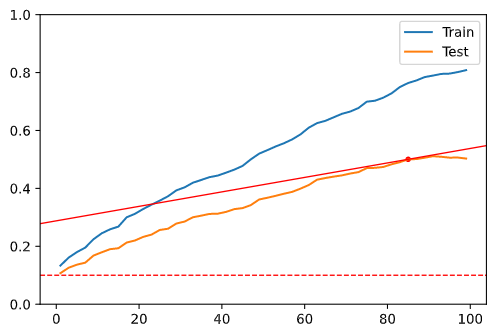
\includegraphics[width=0.5\linewidth]{img/ch5/multi/random.png}
    \caption{Random}
    \label{fig:ch5.multi.random}
\end{figure}

We have designed four configurations that we will use for model selection. Three of them fix the parameter $k$ in line 11 of algorithm \ref{alg:multi}. The fourth one replaces the whole line with the calculation of the coefficient of variance, which can be defined as $c_v = \frac{\sigma}{\mu}$. Note that for the case where $k = 1.0$ our implementation matches that of \texttt{sklearn}, and for values of $K$ approaching infinity this formulation is equivalent to calculating the maximum.

Figure \ref{fig:ch5.multi.plot1} illustrates the performances of the four experiments. Table \ref{fig:ch5.multi.table} holds the specific values for comparison. Note how the best parameter for $k$ is not always 1.0 but shifts to this value as $C$ decreases.

\begin{figure}[h]
    \centering
    \begin{subfigure}[b]{0.4\linewidth}
        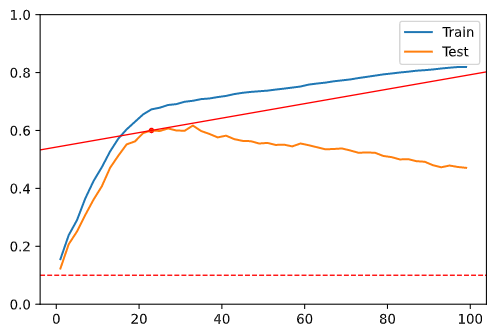
\includegraphics[width=\linewidth]{img/ch5/multi/w-l1.png}
        \subcaption*{$k=0.3$}
    \end{subfigure}
    \begin{subfigure}[b]{0.4\linewidth}
        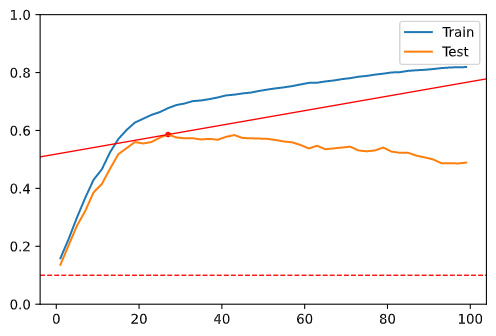
\includegraphics[width=\linewidth]{img/ch5/multi/w-l2.png}
        \subcaption*{$k=1.0$}
    \end{subfigure}
    \begin{subfigure}[b]{0.4\linewidth}
        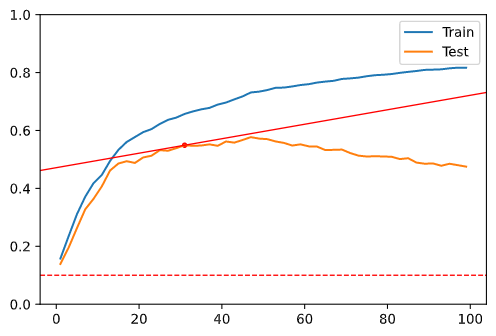
\includegraphics[width=\linewidth]{img/ch5/multi/w-l3.png}
        \subcaption*{$k=3$}
    \end{subfigure}
    \begin{subfigure}[b]{0.4\linewidth}
        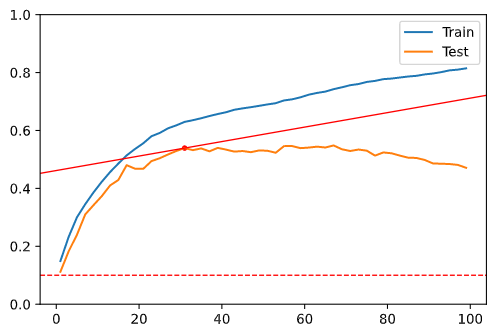
\includegraphics[width=\linewidth]{img/ch5/multi/w-coef.png}
        \subcaption*{Coef. of var.}
    \end{subfigure}
    \caption{SVM-RFE ranking performance with C=0.5 for the multi-class problem.}
    \label{fig:ch5.multi.plot1}
\end{figure}

For this experiment we've calculated the standard error of the cost. In this thesis the cost is usually calculated over the mean of the accuracies and only one value is obtained. In order to provide a standard error, this time we've calculated the cost independently and performed the mean of the costs. Note that due to scalarization both results are not equivalent.

\begin{table}[h]
    \centering
    \makebox[0cm]{
    \begin{tabular}{l | c c c|c c c|c c c}
        \toprule
        \multicolumn{1}{c}{k} & \multicolumn{3}{c}{\textbf{0.3}} & \multicolumn{3}{c}{\textbf{1.0}} & \multicolumn{3}{c}{\textbf{3.0}}\\
        %\cline{2-4}\cline{5-7}\cline{8-10}
        \midrule
        \textbf{$C$}&Feat.&Acc.&Cost&Feat.&Acc.&Cost&Feat.&Acc.&Cost \\
        \midrule
        \textbf{0.05} &    21 & 62.50\% & 0.324 $\pm$ 0.009 &    \mrk{19} & \mrk{62.40\%} & \mrk{0.316} $\pm$ 0.009 &    19 & 62.60\% & 0.322 $\pm$ 0.010\\
        \textbf{0.10} &    21 & 61.81\% & 0.329 $\pm$ 0.011 &    21 & 62.48\% & 0.321 $\pm$ 0.012 &    23 & 62.50\% & 0.320 $\pm$ 0.012\\
        \textbf{0.20} &    21 & 62.49\% & 0.328 $\pm$ 0.009 &    23 & 61.89\% & 0.327 $\pm$ 0.013 &    23 & 60.02\% & 0.347 $\pm$ 0.010\\
        \textbf{0.50} &    23 & 59.48\% & 0.336 $\pm$ 0.011 &    25 & 58.92\% & 0.345 $\pm$ 0.012 &    29 & 53.59\% & 0.390 $\pm$ 0.008\\
        \textbf{1.00} &    23 & 59.22\% & 0.345 $\pm$ 0.013 &    35 & 60.39\% & 0.367 $\pm$ 0.009 &    33 & 53.38\% & 0.395 $\pm$ 0.011\\
        \textbf{2.00} &    29 & 59.40\% & 0.342 $\pm$ 0.013 &    37 & 58.81\% & 0.381 $\pm$ 0.012 &    43 & 56.48\% & 0.402 $\pm$ 0.012\\
        \bottomrule
    \end{tabular}
    }
    \caption{Grid search of SVM-RFE with multi. The cost includes standard error.}
    \label{fig:ch5.multi.table}
\end{table}

\subsubsection*{Digits dataset}

We start with the accuracy of a random ranking (Figure \ref{fig:ch5.multi.digi.random}) to use as a baseline. Then proceed to plot the same four configurations as in the last experiment (Figure \ref{fig:ch5.multi.digit.plot}).

\begin{figure}[h]
    \centering
    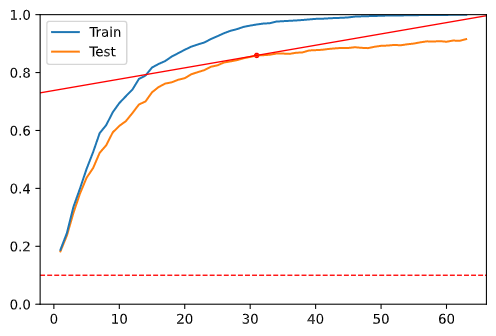
\includegraphics[width=0.4\linewidth]{img/ch5/multi/dig-random.png}
    \caption{Random}
    \label{fig:ch5.multi.digi.random}
\end{figure}

\begin{figure}[h]
    \centering
    \begin{subfigure}[b]{0.4\linewidth}
        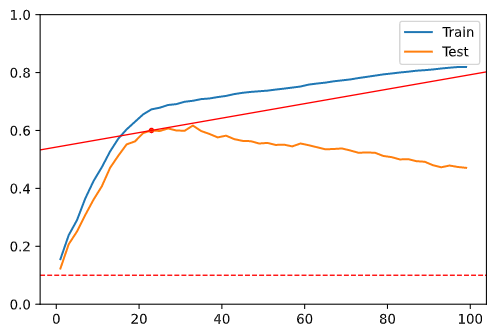
\includegraphics[width=\linewidth]{img/ch5/multi/w-l1.png}
        \subcaption*{$k=0.3$}
    \end{subfigure}
    \begin{subfigure}[b]{0.4\linewidth}
        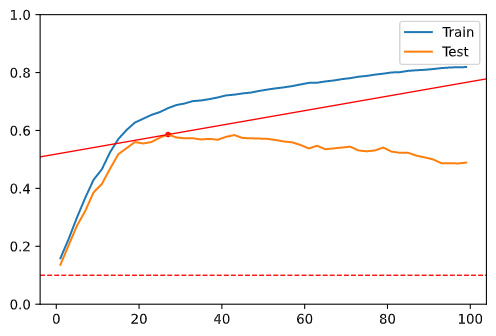
\includegraphics[width=\linewidth]{img/ch5/multi/w-l2.png}
        \subcaption*{$k=1.0$}
    \end{subfigure}
    \begin{subfigure}[b]{0.4\linewidth}
        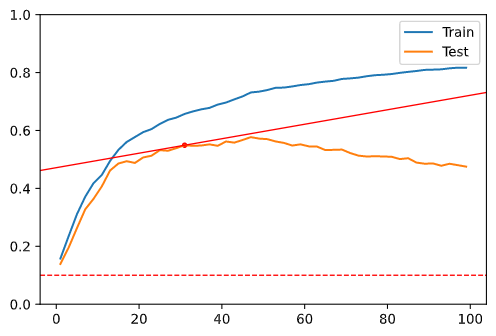
\includegraphics[width=\linewidth]{img/ch5/multi/w-l3.png}
        \subcaption*{$k=3$}
    \end{subfigure}
    \begin{subfigure}[b]{0.4\linewidth}
        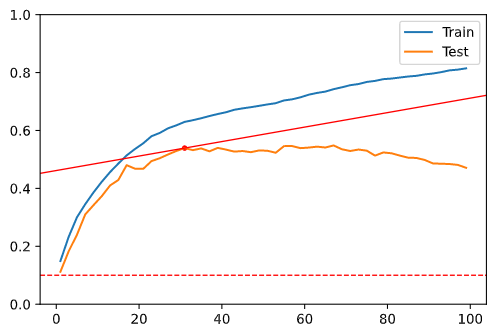
\includegraphics[width=\linewidth]{img/ch5/multi/w-coef.png}
        \subcaption*{Coef. of var.}
    \end{subfigure}
    \caption{SVM-RFE ranking performance with C=0.5 for the digits problem.}
    \label{fig:ch5.multi.digit.plot}
\end{figure}

Table \ref{fig:ch5.multi.digit.table} summarizes the results. We observe that there is not enough difference between cases $k = 0.3$ and $k = 1.0$ to determine if one is better than the other with certainty. 

\begin{table}[H]
    \centering
    \makebox[0cm]{
    \begin{tabular}{l | c c c|c c c|c c c}
        \toprule
        \multicolumn{1}{c}{k} & \multicolumn{3}{c}{\textbf{0.3}} & \multicolumn{3}{c}{\textbf{1.0}} & \multicolumn{3}{c}{\textbf{3.0}}\\
        %\cline{2-4}\cline{5-7}\cline{8-10}
        \midrule
        \textbf{$C$}&Feat.&Acc.&Cost&Feat.&Acc.&Cost&Feat.&Acc.&Cost \\
        \midrule
        \textbf{0.02} &    17 & 93.17\% & 0.097 $\pm$ 0.005 &    17 & 93.30\% & 0.096 $\pm$ 0.004 &    19 & 93.71\% & 0.095 $\pm$ 0.004\\
        \textbf{0.05} &    15 & 91.18\% & 0.101 $\pm$ 0.005 &    19 & 93.24\% & 0.103 $\pm$ 0.004 &    19 & 93.29\% & 0.102 $\pm$ 0.006\\
        \textbf{0.10} &    17 & 92.18\% & 0.102 $\pm$ 0.005 &    \mrk{19} & \mrk{94.29\%} & \mrk{0.094} $\pm$ 0.003 &    19 & 93.65\% & 0.099 $\pm$ 0.003\\
        \textbf{0.20} &    19 & 93.82\% & 0.100 $\pm$ 0.004 &    17 & 92.87\% & 0.098 $\pm$ 0.004 &    19 & 93.00\% & 0.100 $\pm$ 0.003\\
        \textbf{0.50} &    19 & 94.29\% & 0.098 $\pm$ 0.004 &    17 & 92.41\% & 0.099 $\pm$ 0.005 &    19 & 92.83\% & 0.103 $\pm$ 0.005\\
        \textbf{1.00} &    17 & 92.88\% & 0.099 $\pm$ 0.003 &    21 & 94.48\% & 0.098 $\pm$ 0.003 &    19 & 92.88\% & 0.105 $\pm$ 0.004\\
        \textbf{2.00} &    17 & 92.59\% & 0.102 $\pm$ 0.003 &    19 & 93.29\% & 0.103 $\pm$ 0.003 &    19 & 93.47\% & 0.101 $\pm$ 0.004\\
        \bottomrule
    \end{tabular}
    }
    \caption{Grid search of SVM-RFE with multi. The cost includes standard error.}
    \label{fig:ch5.multi.digit.table}
\end{table}

\subsection{Conclusions}

This is a summary of the results for this extension:

\begin{itemize}
    \item Multi-class can be easily implemented in SVM-RFE by using a \emph{sum}.
    \item Using the coefficient of variance produces consistently worse results than the \emph{sum}.
    \item Using a degree $k \neq 1.0$ may reduce the error when the value of $C$ is big, but the results are inconclusive. 
    \item Using a \emph{max} results in worse performance.
\end{itemize}

In general, we recommend using a simple \emph{sum}. Try $k \neq 1.0$ may be a good option when $C \ge 0.5$, but it is not recommended as a first try. 

% --------------------------------------------------------------------------------------------------------------------------------------------
% --------------------------------------------------------------------------------------------------------------------------------------------

\section{Non-linear Kernels}

This extension intends to apply the required modifications in the calculation of the ranking criteria so that non-linear kernels can be used in the SVM.

\subsection{Description and reasoning}
\label{sec:ch5.kernel.desc}

When a problem is not linearly separable, we know that a hard-margin SVM will not be able to correctly place a decision boundary. In this case a soft-margin SVM may be used, but it only works to some extent and if the underlying distribution is near linearly separable. If it is not the case, much better results can be achieved by using non-linear kernels.

To use this method within SVM-RFE we must first be able to compute the ranking coefficient from a non-linear kernel. In contrast with the linear kernel case, where the ranking coefficient can be simplified to $(w_i)^2$, for non-linear kernels, however, since it is a more general case, no simplification can be performed. Instead, we use the general ranking coefficient for SVM (Equation \ref{eq:ch4.grankingcoeff}), which we restate here:
\begin{align*}
    DJ(i) = (1/2)(\boldsymbol{\alpha}^\T \vb{H} \boldsymbol{\alpha} - \boldsymbol{\alpha}^\T \vb{H}(-i) \boldsymbol{\alpha})
\end{align*}

Note that the \emph{hessian} matrix $\vb{H_{i,j}} = y_iy_jk(\vb{x_i}, \vb{x_j})$ needs be computed each iteration (since the dimension of $\vb{x_i}$ and $\vb{x_j}$ will change), and also for each feature removed in each iteration. This is slow. Specifically, since we do have to do an extra loop within RFE for each feature, and require at least $O(mn^2)$ for calculating the Hessian, we know that the complexity will be of $O(m^3n^2)$. However, various optimizations exist, as discussed in the last parts of Section \ref{sec:ch4.rfe.criteria}. The optimizations we are going to implement are:

\subsubsection*{Updating the hessian matrix only for the support vectors}

We know that an observation $i$ that is not a support vector will cause $\alpha_i = 0$. These values are then multiplied by the hessian matrix, but because they are zero they make no contribution to the overall importance calculation. Since we know that they will make no contribution anyway we can also skip recomputing the rows and columns on the Hessian matrix that we know will get multiplied by non-support vectors.

Using a sparse Hessian matrix that only includes support vectors would also work and have the additional benefit of taking less memory to store. However, due to limitations in the \texttt{precomputed} mode of \texttt{sklearn} SVC implementation, we can not do that.

This optimization does not change the overall complexity but may still cause a sig\-ni\-fica\-tive reduction on time in cases where $C$ is small and few support vectors are chosen.

\subsubsection*{Caching previous results}

Depending on the kernel function we may be able to precompute some parts of it if all we want to do is update it for the case where one feature is removed.

Specifically for polynomial kernels we are going to use the following property, which allows us to precompute $\ip{\vb{a}, \vb{b}}$:

\begin{align*}
    \ip{\vb{a}(-i), \vb{b}(-i)} &= \ip{\vb{a}, \vb{b}} - \vb{a}_i \vb{b}_i\\
\end{align*}

And for Gaussian kernels we are going to use the following property, for which we instead need to precompute $\ip{\vb{a} - \vb{b}, \vb{a} - \vb{b}}$:
\begin{align*}
    ||\vb{a}(-i) - \vb{b}(-i)||^2 &= \ip{\vb{a}(-i) - \vb{b}(-i), \vb{a}(-i) - \vb{b}(-i)} \\
    &= \ip{\vb{a} - \vb{b}, \vb{a} - \vb{b}} - (\vb{a}_i - \vb{b}_j )^2
\end{align*}

This optimization allows us to update the Hessian matrix where only one feature is removed in $O(n^2)$, therefore the overall complexity of SVM-RFE becomes $O(m^2n^2)$.

\subsection{Pseudocode formalization}

\begin{algorithm}[H]
    \DontPrintSemicolon
      \KwInput{$t, k$ \tcp*{$t$ = step, $k$ = kernel function}}
      \KwOutput{$\vt{r}$}
      \KwData{$X_0,\vt{y}$}
      $\vt{s} = [1,2, \dotsc, m]$ \tcp*{subset of surviving features}
      $\vt{r} = []$ \tcp*{feature ranking list}
      \While{$|\vt{s}| > 0$}
        {
            \tcc*[h]{Restrict training examples to good feature indices}\\
            $X=X_0(:,\vt{s})$\VS

            \tcc*[h]{Precompute hessian matrix}\\
            $\vb{H_{i,j}} = y_iy_jk(\vb{x_i}, \vb{x_j}) \qquad \text{for all} \qquad \vb{x_i}, \vb{x_j} \in X$\VS

            \tcc*[h]{Train the classifier}\\
            $\vt{\alpha} = \texttt{SVM-train(} X, y, k \texttt{)}$\VS

            \tcc*[h]{Compute the ranking criteria}\\
            $\vt{c} = [c_1, c_2, \dots, c_{|\vt{s}|}]$ \\
            \For{$c_l \in \vt{c}$}{
                \tcc*[h]{Compute new hessian with the feature $l$ removed}\\
                $\vb{H_{i,j}}(-l) = y_iy_jk(\vb{x_i}, \vb{x_j}) \qquad \text{for all} \qquad \vb{x_i}, \vb{x_j} \in X(-l)$\VS
    
                \tcc*[h]{Calculate ranking coefficient}\\
                $c_l = (1/2)(\boldsymbol{\alpha}^\T \vb{H} \boldsymbol{\alpha} - \boldsymbol{\alpha}^\T \vb{H}(-l) \boldsymbol{\alpha})$
            }\VS

            \tcc*[h]{Find the $t$ features with the smallest ranking criterion}\\
            $\vt{f} = \texttt{argsort}(\vt{c})(\ :t)$\VS

            \tcc*[h]{Iterate over the feature subset}\\
            \For{$f_i \in \vt{f}$}{
                \tcc*[h]{Update the feature ranking list}\\
                $\vt{r} = [\vt{s}(f_i), ...\vt{r}]$\VS
    
                \tcc*[h]{Eliminate the feature selected}\\
                $\vt{s} = [...\vt{s}(1:f_i - 1), ...\vt{s}(f_i + 1:|\vt{s}|)]$
            }
        }
    \caption{SVM-RFE with general Kernel}
    \label{alg:ch5.pseudo.kernel}
\end{algorithm}

\subsection{Results}

\subsubsection*{Notes on the implementation}

Using non-linear kernels requires a change in the underlying implementation we've been using for SVM. Until now, we've been relying on the \texttt{LinearSVC} class pro\-vid\-ed by \texttt{Sklearn}, this implementation is in turn based on the \texttt{LIBLINEAR} im\-ple\-men\-ta\-tion for SVM written by the \emph{National Taiwan University}. The authors state that this solver is much faster than the more general version, thus the reason we've been using it, but it can only handle linear kernels. The general version, \texttt{LIBSVM}, created by the same team, is the alternative we're going to use instead. Because now we need to switch, it is interesting to see what will be the increase in computational cost, shown in the table \ref{ch5.kernels.tc1}.

For this first test we've generated artificial datasets with 100 features each, 20 which are informative. Because we want to test the differences with the linear kernel we've used 6 clusters per class, this makes the problem more difficult for lineal separators. 

The following table makes a time comparison using different amount of samples. These are the elapsed times that take completing a validation round using a random ranking. This is similar to RFE without the ranking criteria computations. We've not used SVM-RFE here because we want to demonstrate how the change on the underlying implementation, and not the change in our algorithm, is already a cause for slow down.

\begin{table}[h]
    \centering
    \begin{tabular}{l c c c}
        \toprule
        Obs. & \texttt{LIBLINEAR} & \texttt{LIBSVM} \emph{Linear} & \texttt{LIBSVM} \emph{Precomputed} \\
        \midrule
        500 & 02.67s & 08.17s — x0.32 & 12.04s — x0.22 \\
        1000 & 02.94s & 17.30s — x0.17 & 23.84s — x0.12 \\
        2000 & 04.28s & 43.96s — x0.10 & 50.36s — x0.08 \\
        \bottomrule
        \end{tabular}
    \caption{Cost in time and speedup of a random selection under different implementations and sample sizes.}
    \label{ch5.kernels.tc1}
\end{table}

Note that the sample size increases the cost more than linearly, this may suggest that methods such as dynamic sampling can perform even better than with the \texttt{LIBLINEAR} implementation.

We also note that passing a precomputed kernel matrix (\emph{Gramm} matrix) instead of letting \texttt{sklearn} compute it internally, also increases the time. This is likely an implementation detail, and it is not significant enough to require further in\-ves\-ti\-ga\-tion.

We now plot some examples to compare differences in accuracy (Figure \ref{fig:ch5.kernel.cmp1}). Note that the precomputed kernel, which is a degree-3 polynomial kernel, performs much better at the start. Thus, we can expect it to also perform significantly better with SVM-RFE. 

We can appreciate some differences between the two linear kernels, but they're still clearly following the same curve, which indicates that both implementations are equivalent.  

\begin{figure}[h]
    \centering
    \begin{subfigure}[b]{0.32\linewidth}
        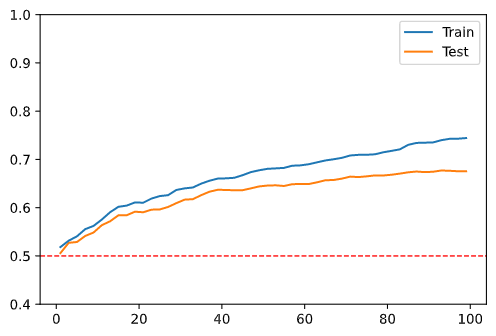
\includegraphics[width=\linewidth]{img/ch5/kernel/random_liblinarl.png}
        \subcaption*{\texttt{LIBLINEAR}}
    \end{subfigure}
    \begin{subfigure}[b]{0.32\linewidth}
        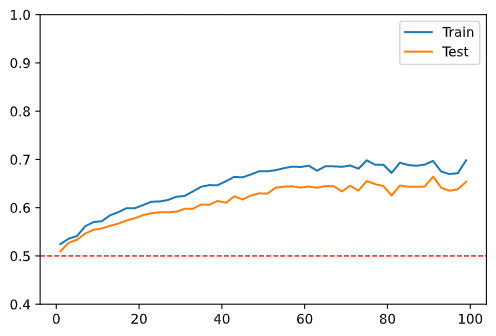
\includegraphics[width=\linewidth]{img/ch5/kernel/random_linar.png}
        \subcaption*{\texttt{LIBSVM} \emph{Linear}}
    \end{subfigure}
    \begin{subfigure}[b]{0.32\linewidth}
        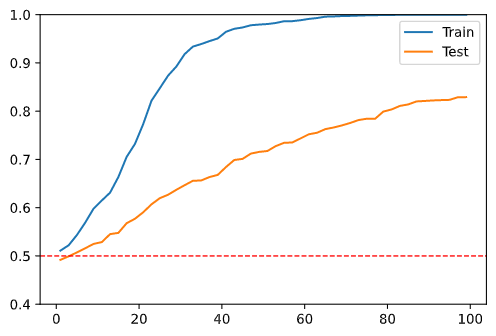
\includegraphics[width=\linewidth]{img/ch5/kernel/random_precomputed.png}
        \subcaption*{\texttt{LIBSVM} \emph{Precomputed}}
    \end{subfigure}
    \caption{Comparison of random selection with 2000 observations.}
    \label{fig:ch5.kernel.cmp1}
\end{figure}

\subsubsection*{Analysis with artificially generated data}
\label{sec:ch5.kernel.art}

We generate a 2 class dataset with the following code.  The scalarization trade-off used is 80\% accuracy, 20\% feature subset size. All results are mean values extracted form a 7-fold cross-validation procedure. We've used a constant step of 10 for SVM-RFE and X for validation.

\begin{verbatim}
    X, y = make_classification(
        n_samples = 500, n_clusters_per_class = 10, n_features = 300, 
        n_informative = 100, n_redundant = 100, n_repeated = 0,
        random_state=2, flip_y= 0.01, class_sep = 3
    )
\end{verbatim}

As usual, we start by plotting the accuracy performance for a random ranking. Note that for this plot the validation is still a SVM with a linear kernel.

\begin{figure}[h]
    \centering
    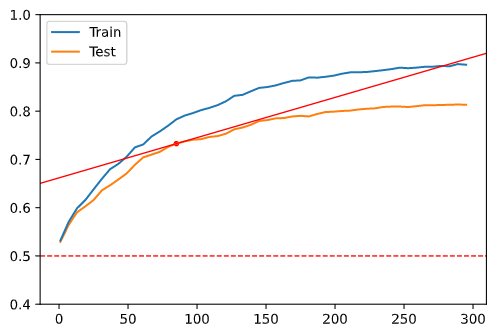
\includegraphics[width=0.4\linewidth]{img/ch5/kernel/art_random.png}
    \caption{Random}
    \label{fig:ch5.kernel.random}
\end{figure}

We observe experimentally in figure \ref{fig:ch5.kernel.cmp2} that, for this dataset, using a non-lineal kernel improves the accuracy of SVM-RFE. Table \ref{fig:ch5.kernel.art.table} summarizes the results from the model selection phase.

\begin{figure}[H]
    \centering
    \begin{subfigure}[b]{0.4\linewidth}
        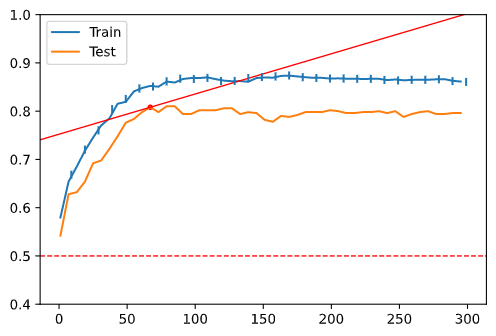
\includegraphics[width=\linewidth]{img/ch5/kernel/art_linear.png}
        \subcaption*{Linear. $C = 0.001$}
    \end{subfigure}
    \begin{subfigure}[b]{0.4\linewidth}
        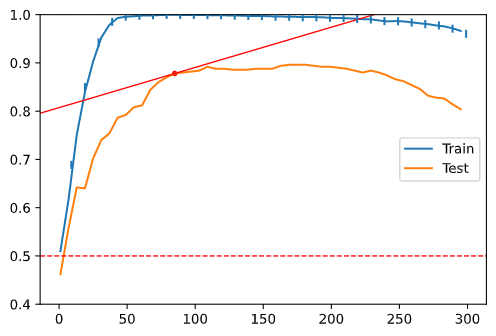
\includegraphics[width=\linewidth]{img/ch5/kernel/art_poly.png}
        \subcaption*{Poly-2. $C = 10^{-6}$}
    \end{subfigure}
    \caption{Accuracy of SVM-RFE feature rankings with the best found regularization coefficient $C$ for linear and polynomial kernels.}
    \label{fig:ch5.kernel.cmp2}
\end{figure}

Non-lineal kernels also involve more hyper-parameters, thus increasing the im\-por\-tance of model selection. The choice of kernel is in itself a hyper-parameter. If a polynomial kernel is chosen then the \emph{degree} and \emph{coefficient} are also hyper-parameters, if a Gaussian kernel is chosen then \emph{gamma}.

\begin{table}[H]
    \centering
    \makebox[0cm]{
    \begin{tabular}{l | c c c|c c c|c c c}
        \toprule
        \multicolumn{1}{c}{deg.} & \multicolumn{3}{c}{\textbf{1}} & \multicolumn{3}{c}{\textbf{2}} & \multicolumn{3}{c}{\textbf{3}}\\
        %\cline{2-4}\cline{5-7}\cline{8-10}
        \midrule
        \textbf{$C$}&Feat.&Acc.&Cost&Feat.&Acc.&Cost&Feat.&Acc.&Cost \\
        \midrule
        \textbf{1e-10} &     1 & 42.40\% & 0.461 &     1 & 46.60\% & 0.428 &    55 & 66.73\% & 0.303\\
        \textbf{1e-09} &     1 & 43.41\% & 0.453 &     1 & 48.80\% & 0.410 &   127 & 79.99\% & 0.245\\
        \textbf{1e-08} &    13 & 54.15\% & 0.375 &     1 & 55.40\% & 0.357 &   115 & 84.39\% & 0.202\\
        \textbf{1e-07} &     1 & 47.20\% & 0.423 &    67 & 82.21\% & 0.187 &    97 & 79.20\% & 0.231\\
        \textbf{1e-06} &     1 & 47.41\% & 0.421 &    \mrk{85} & \mrk{87.81\%} & \mrk{0.154} &   127 & 83.00\% & 0.221\\
        \textbf{1e-05} &     7 & 61.59\% & 0.312 &    79 & 86.82\% & 0.158 &   145 & 84.98\% & 0.217\\
        \textbf{1e-04} &    43 & 76.22\% & 0.219 &    79 & 86.19\% & 0.163 &   151 & 85.19\% & 0.219\\
        \textbf{1e-03} &    67 & 80.81\% & 0.198 &    73 & 85.18\% & 0.167 &   109 & 81.98\% & 0.217\\
        \textbf{1e-02} &    55 & 79.58\% & 0.200 &    85 & 87.60\% & 0.156 &   175 & 87.59\% & 0.216\\
        \textbf{1e-01} &    85 & 82.39\% & 0.198 &    73 & 86.18\% & 0.159 &   109 & 83.39\% & 0.206\\
        \bottomrule
    \end{tabular}
    }
    \caption{Grid search of SVM-RFE with polynomial kernel.}
    \label{fig:ch5.kernel.art.table}
\end{table}

\begin{table}[H]
    \centering
    \begin{tabular}{l | c c c | c c c}
        \toprule
         & \multicolumn{3}{c}{\textbf{Optimized}} & \multicolumn{3}{c}{\textbf{Not optimized}} \\
        %\cline{2-4}\cline{5-7}\cline{8-10}
        \midrule
        \textbf{$C$/Deg.}&\textbf{1}&\textbf{2}&\textbf{3}&\textbf{1}&\textbf{2}&\textbf{3} \\
        \midrule
        \textbf{1e-10} & 0:19.509 & 0:21.968 & 0:22.364     & 0:47.609 & 0:48.374 & 1:16.220\\
        \textbf{1e-09} & 0:21.554 & 0:22.573 & 0:22.636     & 0:51.182 & 0:48.316 & 1:13.988\\
        \textbf{1e-08} & 0:21.617 & 0:22.506 & 0:22.221     & 0:49.338 & 0:53.185 & 1:15.945\\
        \textbf{1e-07} & 0:21.705 & 0:22.073 & 0:21.914     & 0:49.022 & 0:52.526 & 1:08.661\\
        \textbf{1e-06} & 0:21.588 & \mrk{0:20.976} & 0:21.411     & 0:51.579 & \mrk{0:54.387} & 1:07.181\\
        \textbf{1e-05} & 0:21.426 & 0:18.521 & 0:21.937     & 0:53.271 & 0:53.834 & 1:06.723\\
        \textbf{1e-04} & 0:21.513 & 0:19.455 & 0:21.622     & 0:49.130 & 0:50.594 & 1:07.257\\
        \textbf{1e-03} & 0:16.416 & 0:19.160 & 0:22.190     & 0:50.915 & 0:50.858 & 1:06.532\\
        \textbf{1e-02} & 0:13.730 & 0:19.116 & 0:21.048     & 0:48.972 & 0:48.041 & 1:06.149\\
        \textbf{1e-01} & 0:14.009 & 0:18.330 & 0:21.039     & 0:52.361 & 0:47.305 & 1:06.022\\
        \bottomrule
        \end{tabular}
    \caption{Execution time of SVM-RFE with non-linear kernels.}
    \label{fig:ch5.kernel.art.tabletime}
\end{table}

Table \ref{fig:ch5.kernel.art.tabletime} allows us to get an idea of what is the reduction in time we can get with the optimizations described in section \ref{sec:ch5.kernel.desc}. With this information we calculate a speed-up of roughly x3. For the implementation of the optimizations we've used the \texttt{numba} library. This library seamlessly compiles Python functions and allows our optimized Python implementation to compete in speed with the low-level, but not optimized, implementation used by \texttt{sklearn}. We suspect that this automatic Python compilation is not as good as a low-level implementation, therefore it is expected that a low-level implementation of SVM-RFE would be able to produce even more time reduction. 

\subsubsection*{Analysis with MADELON}

The scalarization trade-off used is 80\% accuracy, 20\% feature subset size. All results are mean values extracted form a 7-fold cross-validation procedure. We're using a constant step of 20 for SVM-RFE and 2 for the validation phase. We've normalized the data as a preprocessing step.

Figure \ref{fig:ch5.kernel.cmp3} compares the accuracy performance when a non-linear kernel is used within SVM-RFE versus only in the validation phase. For a comparison with a linear SVM validation phase go back to Figure \ref{fig:ch5.dstep.madelon.rand}.

\begin{figure}[H]
    \centering
    \begin{subfigure}[b]{0.32\linewidth}
        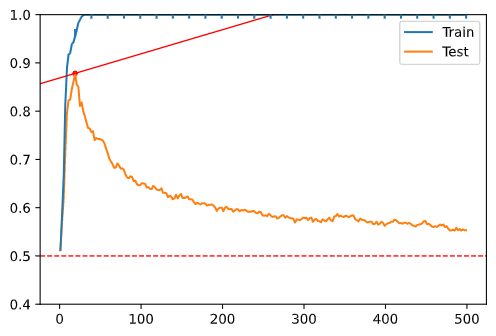
\includegraphics[width=\linewidth]{img/ch5/kernel/mad-t-poly.png}
        \subcaption*{SVM-RFE and validation.}
    \end{subfigure}
    \begin{subfigure}[b]{0.32\linewidth}
        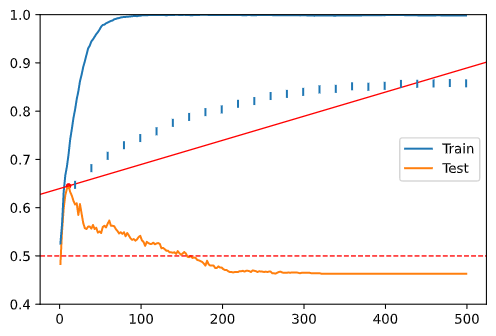
\includegraphics[width=\linewidth]{img/ch5/kernel/mad-t-poly2.png}
        \subcaption*{Only validation.}
    \end{subfigure}
    \begin{subfigure}[b]{0.32\linewidth}
        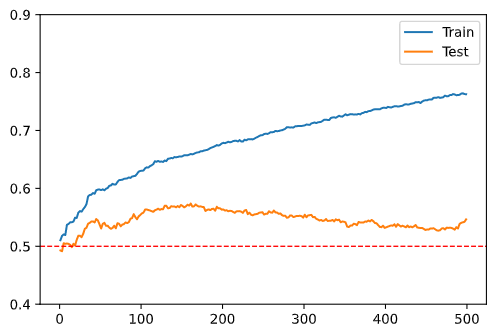
\includegraphics[width=\linewidth]{img/ch5/madelon-random-c_1}
        \subcaption*{All linear.}
    \end{subfigure}
    \caption{Accuracy of SVM-RFE feature rankings with the best found regularization coefficient $C$ for linear and poly-7 kernels. Non-linear validation phases consist of SVM with a Poly-7 kernel.}
    \label{fig:ch5.kernel.cmp3}
\end{figure}

Tables \ref{fig:ch5.kernel.madelon.table} and \ref{fig:ch5.kernel.madelon.timetable} describe the model selection phase for polynomial kernels.

\begin{table}[h]
    \centering
    \makebox[0cm]{
    \begin{tabular}{l | c c c|c c c|c c c}
        \toprule
        \multicolumn{1}{c}{deg.} & \multicolumn{3}{c}{\textbf{1}} & \multicolumn{3}{c}{\textbf{2}} & \multicolumn{3}{c}{\textbf{3}}\\
        %\cline{2-4}\cline{5-7}\cline{8-10}
        \midrule
        \textbf{$C$}&Feat.&Acc.&Cost&Feat.&Acc.&Cost&Feat.&Acc.&Cost \\
        \midrule
        \textbf{0.1} &   123 & 56.83\% & 0.349 $\pm$ 0.013 &    21 & 69.67\% & 0.242 $\pm$ 0.010 &    21 & 74.26\% & 0.211 $\pm$ 0.014\\
        \textbf{0.2} &    67 & 55.75\% & 0.344 $\pm$ 0.014 &    21 & 69.58\% & 0.241 $\pm$ 0.011 &    21 & 76.50\% & 0.192 $\pm$ 0.008\\
        \textbf{0.3} &    49 & 54.66\% & 0.334 $\pm$ 0.013 &    21 & 70.58\% & 0.238 $\pm$ 0.020 &    21 & 77.41\% & 0.183 $\pm$ 0.010\\
        \textbf{0.4} &    31 & 54.67\% & 0.343 $\pm$ 0.015 &    19 & 71.17\% & 0.231 $\pm$ 0.007 &    19 & 77.67\% & 0.175 $\pm$ 0.013\\
        \textbf{0.5} &    11 & 54.24\% & 0.338 $\pm$ 0.018 &    19 & 70.67\% & 0.231 $\pm$ 0.010 &    21 & 77.91\% & 0.183 $\pm$ 0.017\\
        \textbf{0.6} &    57 & 55.51\% & 0.346 $\pm$ 0.012 &    21 & 71.75\% & 0.225 $\pm$ 0.011 &    21 & 78.42\% & 0.170 $\pm$ 0.007\\
        \textbf{0.7} &    59 & 53.42\% & 0.355 $\pm$ 0.013 &    21 & 72.08\% & 0.225 $\pm$ 0.009 &    21 & 78.42\% & 0.174 $\pm$ 0.007\\
        \textbf{0.8} &    27 & 56.25\% & 0.338 $\pm$ 0.011 &    17 & 70.50\% & 0.226 $\pm$ 0.011 &    21 & 77.59\% & 0.177 $\pm$ 0.010\\
        \textbf{0.9} &    25 & 53.76\% & 0.356 $\pm$ 0.006 &    19 & 71.33\% & 0.223 $\pm$ 0.010 &    19 & 78.25\% & 0.178 $\pm$ 0.005\\
        \bottomrule
        \toprule
        \multicolumn{1}{c}{\textbf{deg.}} & \multicolumn{3}{c}{\textbf{4}} & \multicolumn{3}{c}{\textbf{5}} & \multicolumn{3}{c}{\textbf{6}}\\
        %\cline{2-4}\cline{5-7}\cline{8-10}
        \midrule
        \textbf{C}&Feat.&Acc.&Cost&Feat.&Acc.&Cost&Feat.&Acc.&Cost \\
        \midrule
        \textbf{0.1} &    21 & 74.25\% & 0.212 $\pm$ 0.013 &    19 & 74.34\% & 0.212 $\pm$ 0.013 &    19 & 71.00\% & 0.235 $\pm$ 0.011\\
        \textbf{0.2} &    21 & 80.91\% & 0.159 $\pm$ 0.006 &    19 & 81.16\% & 0.154 $\pm$ 0.006 &    19 & 79.75\% & 0.170 $\pm$ 0.014\\
        \textbf{0.3} &    19 & 82.75\% & 0.141 $\pm$ 0.010 &    19 & 84.66\% & 0.128 $\pm$ 0.011 &    21 & 83.08\% & 0.137 $\pm$ 0.014\\
        \textbf{0.4} &    19 & 83.67\% & 0.133 $\pm$ 0.004 &    21 & 86.42\% & 0.113 $\pm$ 0.007 &    19 & 85.41\% & 0.121 $\pm$ 0.007\\
        \textbf{0.5} &    21 & 84.17\% & 0.131 $\pm$ 0.010 &    21 & 86.25\% & 0.116 $\pm$ 0.011 &    19 & 86.49\% & 0.112 $\pm$ 0.008\\
        \textbf{0.6} &    19 & 84.08\% & 0.135 $\pm$ 0.012 &    19 & 85.67\% & 0.117 $\pm$ 0.009 &    19 & 86.76\% & 0.105 $\pm$ 0.009\\
        \textbf{0.7} &    19 & 84.50\% & 0.129 $\pm$ 0.004 &    19 & 86.67\% & 0.111 $\pm$ 0.009 &    19 & 87.00\% & 0.110 $\pm$ 0.010\\
        \textbf{0.8} &    19 & 84.33\% & 0.130 $\pm$ 0.007 &    17 & 85.50\% & 0.113 $\pm$ 0.005 &    19 & 86.75\% & 0.107 $\pm$ 0.006\\
        \textbf{0.9} &    19 & 84.84\% & 0.127 $\pm$ 0.008 &    19 & 85.76\% & 0.117 $\pm$ 0.010 &    19 & 86.58\% & 0.109 $\pm$ 0.003\\
        \bottomrule
        \toprule
        \multicolumn{1}{c}{\textbf{deg.}} & \multicolumn{3}{c}{\textbf{7}} & \multicolumn{3}{c}{\textbf{8}} & \multicolumn{3}{c}{\textbf{9}}\\
        %\cline{2-4}\cline{5-7}\cline{8-10}
        \midrule
        \textbf{C}&Feat.&Acc.&Cost&Feat.&Acc.&Cost&Feat.&Acc.&Cost \\
        \midrule
        \textbf{0.1} &    19 & 69.17\% & 0.240 $\pm$ 0.011 &    17 & 66.84\% & 0.258 $\pm$ 0.010 &    15 & 64.90\% & 0.261 $\pm$ 0.025\\
        \textbf{0.2} &    15 & 70.58\% & 0.218 $\pm$ 0.009 &     7 & 60.93\% & 0.295 $\pm$ 0.026 &     7 & 55.66\% & 0.332 $\pm$ 0.011\\
        \textbf{0.3} &    11 & 72.00\% & 0.205 $\pm$ 0.022 &     7 & 65.09\% & 0.265 $\pm$ 0.031 &     7 & 55.76\% & 0.321 $\pm$ 0.018\\
        \textbf{0.4} &    19 & 86.09\% & 0.116 $\pm$ 0.005 &     9 & 69.19\% & 0.232 $\pm$ 0.032 &     5 & 66.08\% & 0.262 $\pm$ 0.018\\
        \textbf{0.5} &    \mrk{19} & \mrk{88.41\%} & \mrk{0.100 $\pm$ 0.004} &    19 & 86.16\% & 0.113 $\pm$ 0.011 &     7 & 66.68\% & 0.240 $\pm$ 0.014\\
        \textbf{0.6} &    19 & 87.58\% & 0.106 $\pm$ 0.005 &    19 & 87.34\% & 0.104 $\pm$ 0.006 &    17 & 82.08\% & 0.129 $\pm$ 0.013\\
        \textbf{0.7} &    19 & 87.00\% & 0.104 $\pm$ 0.007 &    19 & 87.26\% & 0.107 $\pm$ 0.007 &    19 & 87.08\% & 0.107 $\pm$ 0.010\\
        \textbf{0.8} &    19 & 86.92\% & 0.106 $\pm$ 0.004 &    19 & 86.17\% & 0.109 $\pm$ 0.008 &    19 & 85.92\% & 0.113 $\pm$ 0.004\\
        \textbf{0.9} &    19 & 86.16\% & 0.111 $\pm$ 0.008 &    19 & 85.75\% & 0.110 $\pm$ 0.011 &    19 & 85.75\% & 0.117 $\pm$ 0.006\\
        \bottomrule
    \end{tabular}
    }
    \caption{Grid search of SVM-RFE with polynomial kernel.}
    \label{fig:ch5.kernel.madelon.table}
\end{table}

\begin{table}[h]
    \centering
    \makebox[0cm]{
    \begin{tabular}{l | c c c|c c c|c c c}
        \toprule
        \multicolumn{1}{c}{\textbf{C/deg.}} & \textbf{1} & \textbf{2} & \textbf{3} & \textbf{4} & \textbf{5} & \textbf{6} & \textbf{7} & \textbf{8} & \textbf{9} \\
        %\cline{2-4}\cline{5-7}\cline{8-10}
        \midrule
        \textbf{0.1} & 2:06.42 & 2:05.38 & 2:06.95 & 2:12.24 & 2:13.10 & 2:14.76 & 2:11.08 & 2:17.51 & 2:17.33\\
        \textbf{0.2} & 2:07.59 & 2:04.58 & 2:06.57 & 2:12.31 & 2:12.88 & 2:12.93 & 2:12.17 & 2:17.10 & 2:24.43\\
        \textbf{0.3} & 1:55.10 & 2:04.76 & 2:07.29 & 2:11.48 & 2:12.93 & 2:12.88 & 2:11.95 & 2:16.58 & 2:17.76\\
        \textbf{0.4} & 1:55.69 & 2:01.94 & 2:07.51 & 2:13.60 & 2:12.26 & 2:13.43 & 2:10.84 & 2:16.53 & 2:17.77\\
        \textbf{0.5} & 1:52.74 & 2:01.71 & 2:07.26 & 2:11.87 & 2:13.73 & 2:13.98 & \mrk{2:11.35} & 2:17.51 & 2:17.31\\
        \textbf{0.6} & 1:52.05 & 2:01.22 & 2:06.24 & 2:11.54 & 2:12.87 & 2:13.46 & 2:10.76 & 2:17.58 & 2:16.56\\
        \textbf{0.7} & 1:51.70 & 1:59.91 & 2:05.55 & 2:11.61 & 2:12.28 & 2:13.21 & 2:11.43 & 2:16.34 & 2:16.19\\
        \textbf{0.8} & 1:50.38 & 1:57.42 & 2:05.32 & 2:12.67 & 2:12.39 & 2:15.10 & 2:09.23 & 2:17.35 & 2:18.27\\
        \textbf{0.9} & 1:48.50 & 1:58.06 & 2:03.74 & 2:11.86 & 2:11.66 & 2:12.94 & 2:11.02 & 2:17.79 & 2:16.37\\
        \bottomrule
    \end{tabular}
    }
    \caption{Execution time (min:sec) of SVM-RFE with Polynomial Kernel optimized.}
    \label{fig:ch5.kernel.madelon.timetable}
\end{table}

\subsection{Conclusions}

This is a summary of the results for this extension:

\begin{itemize}
    \item For datasets that are fundamentally not linearly separable, using non-linear kernels produces a huge improvement in accuracy.
    \item Using non-linear kernels is slow, it makes the ranking criteria calculation re\-quire an extra loop and become the bottleneck.
    \item Optimizations improve the cost of the ranking criteria calculation.
    \item Calculations could be potentially made even faster by using a compiled im\-ple\-men\-ta\-tion. 
\end{itemize}

In general, we recommend using non-linear kernels whenever there is suspicion of the data not being linearly separable. If used, we always recommend im\-ple\-ment\-ing the optimizations described in this section.

\section{Combo}

This extension is a combination of the \emph{Non-linear Kernel}, the \emph{Dynamic Step} and the \emph{Sampling} extensions. Because it is straightforward to combine them, we do not provide here the pseudocode.

\subsection{Description and reasoning}

The three extensions have been selected on the hypothesis that they do not interfere with each other, given that they optimize different parts of the algorithm. We've not included the \emph{Multi-class} extension here because we wanted to test the combination specifically on the Madelon dataset. The \emph{Stop Condition} extension is also not include because it optimizes the validation phase, rather than SVM-RFE itself.

One possible incompatibility of the \emph{Sampling} combined with \emph{Dynamic Step} is that the extra time required to resample is increased on the later iterations due to the shrinking of the step. To avoid this, and other similar inconvenient we've slightly modified the \emph{Dynamic Step} implementation with an extra parameter \emph{dstop}. These parameters design a feature subset size that will be the target of dynamic step (instead of 0), and after which point no resampling will be done (the whole dataset will be used).

\subsection{Results}

\subsubsection*{Analysis with artificially generated data}

We reuse the artificial dataset generated in section \ref{sec:ch5.kernel.art}, as a remainder, this is a 2 class dataset made with the following code.  The scalarization trade-off used is 80\% accuracy, 20\% feature subset size. All results are mean values extracted form a 7-fold cross-validation procedure.

\begin{verbatim}
    X, y = make_classification(
        n_samples = 500, n_clusters_per_class = 10, n_features = 300, 
        n_informative = 100, n_redundant = 100, n_repeated = 0,
        random_state=2, flip_y= 0.01, class_sep = 3
    )
\end{verbatim}

For this experiment we've used a dynamic reflective step with a percentage of 20\%, a minimum step of 5 and centered at 100 features. We've also used internal sampling of 70\%. Figure \ref{fig:ch5.combo.art.comp} compares two rankings with the same parameter set, the left one corresponds to a result from the \emph{Non-linear kernel} extension, the right one from this extension.  

\begin{figure}[H]
    \centering
    \begin{subfigure}[b]{0.4\linewidth}
        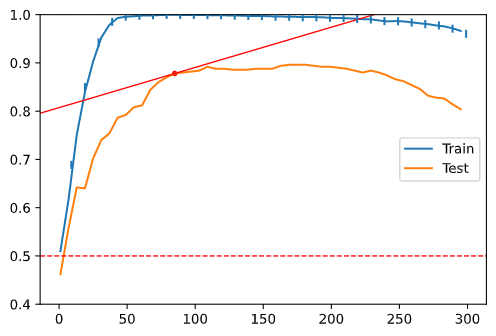
\includegraphics[width=\linewidth]{img/ch5/kernel/art_poly.png}
        \subcaption*{Poly-2. $C = 10^{-6}$}
    \end{subfigure}
    \begin{subfigure}[b]{0.4\linewidth}
        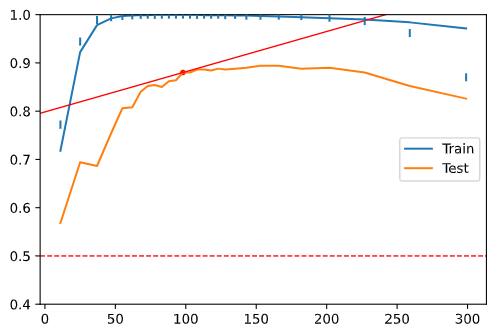
\includegraphics[width=\linewidth]{img/ch5/combo/twice.png}
        \subcaption*{Poly-2. $C = 10^{-6}$}
    \end{subfigure}
    \caption{Performance comparison of SVM-RFE feature rankings. Both show similar accuracy, but the one in the right is twice as fast.}
    \label{fig:ch5.combo.art.comp}
\end{figure}

Tables \ref{fig:ch5.combo.art.table} and \ref{fig:ch5.combo.art.tabletime} summarize the results from this experiment.

\begin{table}[H]
    \centering
    \makebox[0cm]{
    \begin{tabular}{l | c c c|c c c|c c c}
        \toprule
        \multicolumn{1}{c}{deg.} & \multicolumn{3}{c}{\textbf{1}} & \multicolumn{3}{c}{\textbf{2}} & \multicolumn{3}{c}{\textbf{3}}\\
        %\cline{2-4}\cline{5-7}\cline{8-10}
        \midrule
        \textbf{$C$}&Feat.&Acc.&Cost&Feat.&Acc.&Cost&Feat.&Acc.&Cost \\
        \midrule
        \textbf{1e-10} &    11 & 45.01\% & 0.447 &    11 & 46.81\% & 0.433 &    47 & 70.63\% & 0.266\\
        \textbf{1e-09} &    11 & 44.40\% & 0.452 &    11 & 47.00\% & 0.431 &   108 & 82.20\% & 0.214\\
        \textbf{1e-08} &    11 & 45.97\% & 0.440 &    37 & 52.16\% & 0.407 &   113 & 81.79\% & 0.221\\
        \textbf{1e-07} &    11 & 45.40\% & 0.444 &    83 & 82.41\% & 0.196 &   108 & 82.80\% & 0.210\\
        \textbf{1e-06} &    11 & 49.17\% & 0.414 &    98 & 88.01\% & 0.161 &   113 & 82.02\% & 0.219\\
        \textbf{1e-05} &    11 & 66.20\% & 0.278 &    88 & 86.79\% & 0.164 &   108 & 82.20\% & 0.214\\
        \textbf{1e-04} &    37 & 75.61\% & 0.220 &    88 & 86.01\% & 0.171 &   108 & 82.82\% & 0.209\\
        \textbf{1e-03} &    55 & 77.58\% & 0.216 &    83 & 86.59\% & 0.163 &   108 & 81.81\% & 0.218\\
        \textbf{1e-02} &    78 & 82.20\% & 0.194 &    \mrk{83} & \mrk{88.60\%} & \mrk{0.147} &   123 & 82.79\% & 0.220\\
        \textbf{1e-01} &    62 & 77.20\% & 0.224 &    88 & 88.41\% & 0.151 &   143 & 83.81\% & 0.225\\
        \bottomrule
    \end{tabular}
    }
    \caption{Grid search of SVM-RFE with polynomial kernel.}
    \label{fig:ch5.combo.art.table}
\end{table}

\begin{table}[H]
    \centering
    \begin{tabular}{l | c c c}
        \toprule
        \textbf{$C$/Deg.}&\textbf{1}&\textbf{2}&\textbf{3} \\
        \midrule
        \textbf{1e-10} & 0:08.003 & 0:08.314 & 0:08.781\\
        \textbf{1e-09} & 0:07.922 & 0:08.231 & 0:08.670\\
        \textbf{1e-08} & 0:07.928 & 0:08.341 & 0:08.646\\
        \textbf{1e-07} & 0:08.075 & 0:08.506 & 0:08.523\\
        \textbf{1e-06} & 0:08.035 & 0:07.961 & 0:08.453\\
        \textbf{1e-05} & 0:08.198 & 0:07.834 & 0:08.525\\
        \textbf{1e-04} & 0:07.956 & 0:07.739 & 0:08.571\\
        \textbf{1e-03} & 0:06.849 & 0:07.851 & 0:08.461\\
        \textbf{1e-02} & 0:06.134 & \mrk{0:08.189} & 0:08.510\\
        \textbf{1e-01} & 0:05.541 & 0:08.097 & 0:08.582\\
        \bottomrule
        \end{tabular}
    \caption{Execution time of SVM-RFE with non-linear kernels.}
    \label{fig:ch5.combo.art.tabletime}
\end{table}

By comparing this results to Table \ref{fig:ch5.kernel.art.tabletime} we calculate an approximate speed-up of x2 compared to the optimized non-linear kernel version.

We have also tried using a Gaussian kernel (Table \ref{fig:ch5.combo.art.tablerbf}). Although using it we can obtain grater values of accuracy, the amount of features it selects also increase significatively. Overall the RBF kernel doesn't perform as good as the polynomial for this dataset. Note that RBF kernel results for the \emph{Non-lineal kernel} extension are the same and have been omitted. The time table has also been omitted.

\begin{table}[H]
    \centering
    \makebox[0cm]{
    \begin{tabular}{l | c c c|c c c|c c c}
        \toprule
        \multicolumn{1}{c}{$\gamma$} & \multicolumn{3}{c}{\textbf{0.00036}} & \multicolumn{3}{c}{\textbf{0.00046}} & \multicolumn{3}{c}{\textbf{0.00056}}\\
        %\cline{2-4}\cline{5-7}\cline{8-10}
        \midrule
        \textbf{$C$}&Feat.&Acc.&Cost&Feat.&Acc.&Cost&Feat.&Acc.&Cost \\
        \midrule
        \textbf{1e+00} &   161 & 88.41\% & 0.200 &   132 & 85.39\% & 0.205 &   102 & 79.82\% & 0.229 \\
        \textbf{1e+01} &   157 & 91.39\% & 0.174 &   134 & 88.60\% & 0.181 &   104 & 83.01\% & 0.205 \\
        \textbf{1e+02} &   145 & 89.81\% & 0.178 &   134 & 89.01\% & 0.177 &   110 & 86.99\% & 0.177 \\
        \textbf{1e+03} &   \mrk{157} & \mrk{91.59\%} & \mrk{0.172} &   132 & 87.80\% & 0.186 &   102 & 85.79\% & 0.182 \\
        \textbf{1e+04} &   149 & 89.22\% & 0.186 &   134 & 87.39\% & 0.190 &   106 & 81.59\% & 0.218 \\
        \textbf{1e+05} &   161 & 90.01\% & 0.187 &   132 & 87.80\% & 0.186 &   106 & 82.20\% & 0.213 \\
        \bottomrule
    \end{tabular}
    }
    \caption{Grid search of SVM-RFE with RBF kernel.}
    \label{fig:ch5.combo.art.tablerbf}
\end{table}

\subsubsection*{Analysis with MADELON}

For this experiment we've used a dynamic reflective step with a percentage of 8\%, a minimum step of 3 and centered at 20 features. We've also used internal sampling of 20\%. Figure \ref{fig:ch5.combo.madelon.one} corresponds to the feature ranking accuracy with the best pa\-ram\-e\-ters found in the model selection phase.  

\begin{figure}[H]
    \centering
    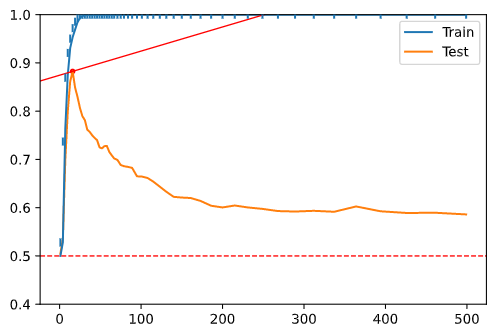
\includegraphics[width=0.4\linewidth]{img/ch5/combo/once.png}
    \caption{Poly-7, $C=0.6$}
    \label{fig:ch5.combo.madelon.one}
\end{figure}

Tables \ref{fig:ch5.combo.madelon.table} and \ref{fig:ch5.combo.madelon.timetable} summarize the results. We note that although we were not able to improve the accuracy compared with the version only with non-polynomial kernels, we've achieved a speed-up of x6.

The following figure (Figure \ref{fig:ch5.combo.art.comp2}) illustrates what happens if we remove either \emph{Dynamic Step} or \emph{Sampling} from our \emph{Combo} extension. Removing internal sampling significatively reduces the accuracy. Using a constant step instead of dynamic also performs worse, either by increasing the elapsed time when a small step is used, or decreasing the accuracy when the value of the step is large. Although the accuracy reduced by using a large step (e.g. 50) is small (3\% drop), it may produce an im\-por\-tant speed up of the SVM-RFE phase. However, the validation phase still requires using dynamic step or a very small constant step to avoid the accuracy performance drop\-ping considerably. 

\begin{figure}[H]
    \centering
    \begin{subfigure}[b]{0.4\linewidth}
        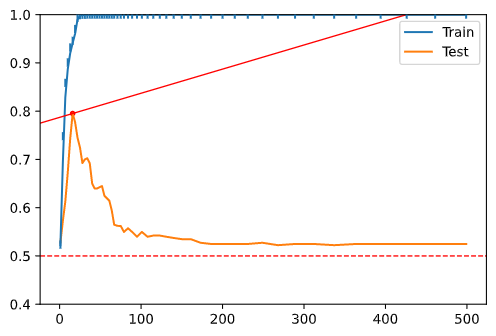
\includegraphics[width=\linewidth]{img/ch5/combo/twice-2.png}
        \subcaption*{Preprocessed sampling of $20\%$}
    \end{subfigure}
    \begin{subfigure}[b]{0.4\linewidth}
        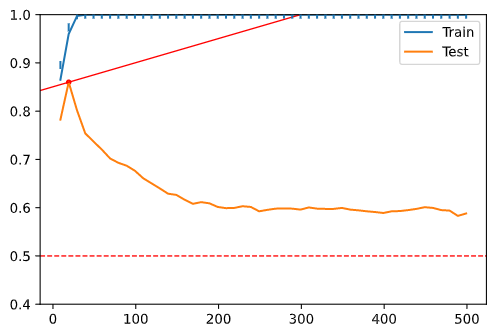
\includegraphics[width=\linewidth]{img/ch5/combo/twice-3.png}
        \subcaption*{Constant step of 10}
    \end{subfigure}
    \caption{Performance comparison of SVM-RFE (Combo) feature rankings with some extension removed. Poly-7, $C=0.6$}
    \label{fig:ch5.combo.art.comp2}
\end{figure}

\begin{table}[h]
    \centering
    \makebox[0cm]{
    \begin{tabular}{l | c c c|c c c|c c c}
        \toprule
        \multicolumn{1}{c}{deg.} & \multicolumn{3}{c}{\textbf{1}} & \multicolumn{3}{c}{\textbf{2}} & \multicolumn{3}{c}{\textbf{3}}\\
        %\cline{2-4}\cline{5-7}\cline{8-10}
        \midrule
        \textbf{$C$}&Feat.&Acc.&Cost&Feat.&Acc.&Cost&Feat.&Acc.&Cost \\
        \midrule
        \textbf{0.1} &    22 & 55.45\% & 0.335 $\pm$ 0.004 &    19 & 69.65\% & 0.245 $\pm$ 0.009 &    19 & 75.40\% & 0.200 $\pm$ 0.011\\
        \textbf{0.2} &    61 & 55.60\% & 0.345 $\pm$ 0.008 &    19 & 71.05\% & 0.235 $\pm$ 0.007 &    19 & 78.50\% & 0.177 $\pm$ 0.008\\
        \textbf{0.3} &    31 & 58.95\% & 0.323 $\pm$ 0.011 &    19 & 71.05\% & 0.228 $\pm$ 0.009 &    19 & 78.15\% & 0.178 $\pm$ 0.005\\
        \textbf{0.4} &    13 & 58.25\% & 0.319 $\pm$ 0.010 &    19 & 71.50\% & 0.232 $\pm$ 0.010 &    22 & 78.20\% & 0.177 $\pm$ 0.008\\
        \textbf{0.5} &    49 & 56.15\% & 0.342 $\pm$ 0.010 &    19 & 71.75\% & 0.222 $\pm$ 0.004 &    19 & 78.65\% & 0.176 $\pm$ 0.006\\
        \textbf{0.6} &    28 & 57.25\% & 0.334 $\pm$ 0.011 &    19 & 71.65\% & 0.227 $\pm$ 0.009 &    19 & 78.65\% & 0.174 $\pm$ 0.007\\
        \textbf{0.7} &    49 & 56.55\% & 0.336 $\pm$ 0.013 &    19 & 71.40\% & 0.228 $\pm$ 0.005 &    19 & 78.85\% & 0.174 $\pm$ 0.008\\
        \textbf{0.8} &    34 & 56.05\% & 0.346 $\pm$ 0.011 &    16 & 71.40\% & 0.229 $\pm$ 0.006 &    19 & 79.10\% & 0.172 $\pm$ 0.005\\
        \textbf{0.9} &    28 & 56.90\% & 0.342 $\pm$ 0.011 &    22 & 70.90\% & 0.234 $\pm$ 0.008 &    19 & 79.60\% & 0.168 $\pm$ 0.011\\
        \bottomrule
        \toprule
        \multicolumn{1}{c}{\textbf{deg.}} & \multicolumn{3}{c}{\textbf{4}} & \multicolumn{3}{c}{\textbf{5}} & \multicolumn{3}{c}{\textbf{6}}\\
        %\cline{2-4}\cline{5-7}\cline{8-10}
        \midrule
        \textbf{C}&Feat.&Acc.&Cost&Feat.&Acc.&Cost&Feat.&Acc.&Cost \\
        \midrule
        \textbf{0.1} &    19 & 77.24\% & 0.183 $\pm$ 0.014 &    16 & 73.60\% & 0.198 $\pm$ 0.021 &    16 & 77.54\% & 0.185 $\pm$ 0.016\\
        \textbf{0.2} &    19 & 83.90\% & 0.135 $\pm$ 0.005 &    19 & 84.15\% & 0.129 $\pm$ 0.009 &    16 & 79.55\% & 0.146 $\pm$ 0.010\\
        \textbf{0.3} &    19 & 84.25\% & 0.130 $\pm$ 0.005 &    19 & 85.55\% & 0.116 $\pm$ 0.008 &    16 & 81.00\% & 0.142 $\pm$ 0.017\\
        \textbf{0.4} &    19 & 83.75\% & 0.135 $\pm$ 0.005 &    19 & 86.85\% & 0.113 $\pm$ 0.006 &    19 & 86.50\% & 0.113 $\pm$ 0.008\\
        \textbf{0.5} &    19 & 84.45\% & 0.130 $\pm$ 0.004 &    19 & 86.75\% & 0.113 $\pm$ 0.007 &    16 & 85.35\% & 0.116 $\pm$ 0.006\\
        \textbf{0.6} &    19 & 84.15\% & 0.132 $\pm$ 0.005 &    19 & 86.90\% & 0.108 $\pm$ 0.008 &    19 & 87.80\% & 0.103 $\pm$ 0.004\\
        \textbf{0.7} &    19 & 84.65\% & 0.130 $\pm$ 0.005 &    19 & 86.65\% & 0.111 $\pm$ 0.005 &    19 & 86.45\% & 0.110 $\pm$ 0.005\\
        \textbf{0.8} &    19 & 84.35\% & 0.132 $\pm$ 0.010 &    19 & 86.85\% & 0.112 $\pm$ 0.007 &    19 & 87.20\% & 0.104 $\pm$ 0.006\\
        \textbf{0.9} &    22 & 85.10\% & 0.123 $\pm$ 0.005 &    19 & 86.65\% & 0.113 $\pm$ 0.006 &    19 & 86.30\% & 0.109 $\pm$ 0.004\\
        \bottomrule
        \toprule
        \multicolumn{1}{c}{\textbf{deg.}} & \multicolumn{3}{c}{\textbf{7}} & \multicolumn{3}{c}{\textbf{8}} & \multicolumn{3}{c}{\textbf{9}}\\
        %\cline{2-4}\cline{5-7}\cline{8-10}
        \midrule
        \textbf{C}&Feat.&Acc.&Cost&Feat.&Acc.&Cost&Feat.&Acc.&Cost \\
        \midrule
        \textbf{0.1} &    16 & 72.45\% & 0.189 $\pm$ 0.012 &    16 & 73.26\% & 0.190 $\pm$ 0.020 &    13 & 71.15\% & 0.223 $\pm$ 0.024\\
        \textbf{0.2} &    13 & 77.80\% & 0.174 $\pm$ 0.027 &    10 & 71.00\% & 0.206 $\pm$ 0.024 &    10 & 65.40\% & 0.258 $\pm$ 0.027\\
        \textbf{0.3} &     7 & 69.00\% & 0.219 $\pm$ 0.026 &     7 & 60.44\% & 0.280 $\pm$ 0.023 &    10 & 58.35\% & 0.318 $\pm$ 0.010\\
        \textbf{0.4} &    10 & 77.60\% & 0.176 $\pm$ 0.023 &     7 & 62.50\% & 0.276 $\pm$ 0.029 &     7 & 62.25\% & 0.284 $\pm$ 0.022\\
        \textbf{0.5} &    13 & 85.65\% & 0.117 $\pm$ 0.012 &    10 & 69.14\% & 0.212 $\pm$ 0.029 &     7 & 65.61\% & 0.258 $\pm$ 0.031\\
        \textbf{0.6} &    \mrk{16} & \mrk{88.25\%} & \mrk{0.098 $\pm$ 0.004} &    10 & 72.20\% & 0.195 $\pm$ 0.025 &    10 & 70.94\% & 0.214 $\pm$ 0.030\\
        \textbf{0.7} &    19 & 87.35\% & 0.105 $\pm$ 0.009 &    13 & 85.50\% & 0.116 $\pm$ 0.008 &    10 & 70.95\% & 0.215 $\pm$ 0.037\\
        \textbf{0.8} &    19 & 87.90\% & 0.104 $\pm$ 0.005 &    16 & 87.05\% & 0.102 $\pm$ 0.005 &    10 & 81.16\% & 0.135 $\pm$ 0.010\\
        \textbf{0.9} &    19 & 87.45\% & 0.106 $\pm$ 0.006 &    19 & 87.05\% & 0.105 $\pm$ 0.004 &    16 & 84.75\% & 0.115 $\pm$ 0.009\\
        \bottomrule
    \end{tabular}
    }
    \caption{Grid search of SVM-RFE (combo) with polynomial kernel.}
    \label{fig:ch5.combo.madelon.table}
\end{table}

\begin{table}[h]
    \centering
    \makebox[0cm]{
    \begin{tabular}{l | c c c|c c c|c c c}
        \toprule
        \multicolumn{1}{c}{\textbf{C/deg.}} & \textbf{1} & \textbf{2} & \textbf{3} & \textbf{4} & \textbf{5} & \textbf{6} & \textbf{7} & \textbf{8} & \textbf{9} \\
        %\cline{2-4}\cline{5-7}\cline{8-10}
        \midrule
        \textbf{0.1} & 0:20.24 & 0:20.80 & 0:20.75 & 0:24.10 & 0:21.58 & 0:21.40 & 0:21.68 & 0:21.64 & 0:20.16\\
        \textbf{0.2} & 0:20.66 & 0:20.78 & 0:20.65 & 0:24.01 & 0:21.97 & 0:21.31 & 0:21.44 & 0:22.25 & 0:20.15\\
        \textbf{0.3} & 0:21.37 & 0:20.61 & 0:20.76 & 0:22.29 & 0:21.52 & 0:21.93 & 0:21.98 & 0:22.16 & 0:21.79\\
        \textbf{0.4} & 0:19.71 & 0:21.18 & 0:20.76 & 0:21.30 & 0:22.64 & 0:21.73 & 0:21.62 & 0:21.83 & 0:22.00\\
        \textbf{0.5} & 0:19.89 & 0:20.43 & 0:21.56 & 0:21.47 & 0:21.46 & 0:21.54 & 0:21.61 & 0:21.87 & 0:22.03\\
        \textbf{0.6} & 0:19.09 & 0:20.13 & 0:20.42 & 0:21.08 & 0:21.39 & 0:21.83 & \mrk{0:21.82} & 0:22.03 & 0:22.24\\
        \textbf{0.7} & 0:19.19 & 0:20.02 & 0:20.83 & 0:21.64 & 0:21.06 & 0:21.61 & 0:21.79 & 0:22.34 & 0:22.05\\
        \textbf{0.8} & 0:19.49 & 0:19.76 & 0:20.97 & 0:21.09 & 0:21.26 & 0:21.62 & 0:21.33 & 0:21.73 & 0:21.92\\
        \textbf{0.9} & 0:19.49 & 0:19.73 & 0:20.39 & 0:21.22 & 0:21.49 & 0:22.12 & 0:21.39 & 0:22.16 & 0:23.06\\
        \bottomrule
    \end{tabular}
    }
    \caption{Execution time (min:sec) of SVM-RFE (combo) with Polynomial Kernel optimized.}
    \label{fig:ch5.combo.madelon.timetable}
\end{table}

We have also tried using a Gaussian kernel (Table \ref{fig:ch5.combo.madelon.table-rbf}). The results are not as good as using a polynomial, but it produces smaller feature subsets. The timetable has been omitted.

\begin{table}[h]
    \centering
    \makebox[0cm]{
    \begin{tabular}{l | c c c|c c c|c c c}
        \toprule
        \multicolumn{1}{c}{$\gamma$} & \multicolumn{3}{c}{\textbf{0.010}} & \multicolumn{3}{c}{\textbf{0.025}} & \multicolumn{3}{c}{\textbf{0.050}}\\
        %\cline{2-4}\cline{5-7}\cline{8-10}
        \midrule
        \textbf{$C$}&Feat.&Acc.&Cost&Feat.&Acc.&Cost&Feat.&Acc.&Cost \\
        \midrule
        \textbf{0.1} &    13 & 61.70\% & 0.308 $\pm$ 0.010 &    19 & 69.05\% & 0.251 $\pm$ 0.009 &    16 & 71.60\% & 0.225 $\pm$ 0.009\\
        \textbf{0.2} &    22 & 63.50\% & 0.295 $\pm$ 0.011 &    22 & 73.05\% & 0.220 $\pm$ 0.009 &    16 & 76.15\% & 0.191 $\pm$ 0.009\\
        \textbf{0.3} &    22 & 65.75\% & 0.271 $\pm$ 0.009 &    22 & 74.50\% & 0.209 $\pm$ 0.006 &    16 & 77.10\% & 0.187 $\pm$ 0.012\\
        \textbf{0.4} &    28 & 68.05\% & 0.264 $\pm$ 0.007 &    22 & 76.40\% & 0.195 $\pm$ 0.003 &    16 & 76.20\% & 0.186 $\pm$ 0.010\\
        \textbf{0.5} &    22 & 68.95\% & 0.251 $\pm$ 0.007 &    22 & 76.70\% & 0.190 $\pm$ 0.006 &    16 & 80.75\% & 0.157 $\pm$ 0.011\\
        \textbf{0.6} &    25 & 69.60\% & 0.243 $\pm$ 0.008 &    19 & 77.50\% & 0.186 $\pm$ 0.007 &    16 & 79.70\% & 0.165 $\pm$ 0.014\\
        \textbf{0.7} &    28 & 71.05\% & 0.239 $\pm$ 0.008 &    22 & 78.35\% & 0.176 $\pm$ 0.007 &    16 & 80.90\% & 0.153 $\pm$ 0.009\\
        \textbf{0.8} &    19 & 69.30\% & 0.244 $\pm$ 0.005 &    22 & 78.45\% & 0.177 $\pm$ 0.010 &    16 & 79.35\% & 0.169 $\pm$ 0.014\\
        \textbf{0.9} &    22 & 70.90\% & 0.235 $\pm$ 0.006 &    22 & 78.75\% & 0.176 $\pm$ 0.008 &    16 & 79.70\% & 0.164 $\pm$ 0.014\\
        \textbf{1.0} &    25 & 71.70\% & 0.228 $\pm$ 0.008 &    19 & 79.60\% & 0.168 $\pm$ 0.010 &    16 & 81.40\% & 0.153 $\pm$ 0.010\\
        \bottomrule
        \toprule
        \multicolumn{1}{c}{$\gamma$} & \multicolumn{3}{c}{\textbf{0.1}} & \multicolumn{3}{c}{\textbf{0.2}} & \multicolumn{3}{c}{\textbf{0.3}}\\
        %\cline{2-4}\cline{5-7}\cline{8-10}
        \midrule
        \textbf{C}&Feat.&Acc.&Cost&Feat.&Acc.&Cost&Feat.&Acc.&Cost \\
        \midrule
        \textbf{0.1} &    16 & 76.10\% & 0.196 $\pm$ 0.012 &     7 & 67.75\% & 0.260 $\pm$ 0.012 &     4 & 57.95\% & 0.333 $\pm$ 0.018\\
        \textbf{0.2} &    13 & 78.30\% & 0.167 $\pm$ 0.009 &     7 & 68.00\% & 0.248 $\pm$ 0.020 &     4 & 58.15\% & 0.324 $\pm$ 0.023\\
        \textbf{0.3} &    13 & 79.90\% & 0.159 $\pm$ 0.012 &     7 & 67.10\% & 0.250 $\pm$ 0.022 &     4 & 60.45\% & 0.310 $\pm$ 0.020\\
        \textbf{0.4} &    13 & 78.95\% & 0.166 $\pm$ 0.010 &     7 & 75.30\% & 0.199 $\pm$ 0.011 &    10 & 56.54\% & 0.337 $\pm$ 0.025\\
        \textbf{0.5} &    13 & 82.60\% & 0.143 $\pm$ 0.005 &     7 & 72.75\% & 0.211 $\pm$ 0.024 &     4 & 60.55\% & 0.310 $\pm$ 0.015\\
        \textbf{0.6} &    13 & 82.95\% & 0.137 $\pm$ 0.012 &     7 & 73.65\% & 0.202 $\pm$ 0.018 &     4 & 64.50\% & 0.276 $\pm$ 0.020\\
        \textbf{0.7} &    13 & 82.15\% & 0.141 $\pm$ 0.009 &     7 & 72.75\% & 0.209 $\pm$ 0.027 &     4 & 56.30\% & 0.330 $\pm$ 0.017\\
        \textbf{0.8} &    13 & 82.40\% & 0.139 $\pm$ 0.007 &     7 & 77.30\% & 0.182 $\pm$ 0.016 &     4 & 62.30\% & 0.299 $\pm$ 0.017\\
        \textbf{0.9} &    13 & 82.75\% & 0.139 $\pm$ 0.010 &     7 & 79.25\% & 0.158 $\pm$ 0.011 &     7 & 55.05\% & 0.343 $\pm$ 0.018\\
        \textbf{1.0} &    13 & 84.50\% & 0.124 $\pm$ 0.011 &     7 & 79.80\% & 0.164 $\pm$ 0.012 &     4 & 58.40\% & 0.314 $\pm$ 0.029\\
        \bottomrule
    \end{tabular}
    }
    \caption{Grid search of SVM-RFE (combo) with RBF kernel.}
    \label{fig:ch5.combo.madelon.table-rbf}
\end{table}

\subsection{Conclusions}

This is a summary of the results for this extension:

\begin{itemize}
    \item As expected, this combo produces a substantial speed-up.
    \item Accuracy is not negatively effected by the new method.
    \item Finding the correct parameters for \emph{Dynamic Step} and \emph{Sampling} requires knowl\-edge on the data. 
\end{itemize}

Although this method requires extra parameters, these have well-defined ranges and are not very sensitive to changes. This makes it possible to find adequate values with a simple initial exploratory analysis without requiring more complex model selection algorithms. 

In general, we recommend using this combo approach whenever the data is not linearly separable and the approximate amount of informative features is known. A previous exploration of the data set may be required.